% Institute of Computer Science thesis template
% authors: Sven Laur, Liina Kamm
% last change Tõnu Tamme 09.05.2017
%--
% Compilation instructions:
% 1. Choose main language on line 55-56 (English or Estonian)
% 2. Compile 1-3 times to get refences right
% pdflatex bachelors-thesis-template
% bibtex bachelors-thesis-template
%--
% Please use references like this:
% <text> <non-breaking-space> <cite/ref-command> <punctuation>
% This is an example~\cite{example}.

\documentclass[12pt]{article}

% A package for setting layout and margins for your thesis 
\usepackage[a4paper]{geometry}

%%=== A4 page setup ===
%\setlength{\paperwidth}{21.0cm} 
%\setlength{\paperheight}{29.7cm}
%\setlength{\textwidth}{16cm}
%\setlength{\textheight}{25cm}


% When you write in Estonian then you want to use text with right character set
% By default LaTeX does not know what to do with õäöu letters. You have to specify
% a correct input and font encoding. For that you have to Google the Web     
%
% For TexShop under MacOS X. The right lines are 
%\usepackage[applemac]{inputenc}
%\usepackage[T1]{fontenc} %Absolutely critical for *hyphenation* of words with non-ASCII letters.
%
% For Windows and Linux the right magic lines are   
% \usepackage[latin1]{inputenc}
% \usepackage[latin5]{inputenc}
%%\usepackage[utf8]{inputenc} %Package inputenc Error: Unicode char ´ (U+B4) not set up for use with LaTeX
\usepackage[utf8x]{inputenc}
\usepackage[T1]{fontenc} %Absolutely critical for *hyphenation* of words with non-ASCII letters.

% Typeset text in Times Roman instead of Computer Modern (EC)
\usepackage{times}

% Suggested packages:
\usepackage{microtype}  %towards typographic perfection...
\usepackage{inconsolata} %nicer font for code listings. (Use \ttfamily for lstinline bastype)


% Use package babel for English or Estonian 
% If you use Estonian make sure that Estonian hyphenation is installed 
% - hypen-estonian or eehyp packages
%
%===Choose the main language in thesis
\usepackage[estonian, english]{babel} %the thesis is in English 
%\usepackage[english, estonian]{babel} %the thesis is in Estonian


% Change Babel document elements 
\addto\captionsestonian{%
  \renewcommand{\refname}{Viidatud kirjandus}%
  \renewcommand{\appendixname}{Lisad}%
}


% If you have problems with Estonian keywords in the bibliography
%\usepackage{biblatex}
%\usepackage[backend=biber]{biblatex}
%\usepackage[style=alphabetic]{biblatex}
% plain --> \usepackage[style=numeric]{biblatex}
% abbrv --> \usepackage[style=numeric,firstinits=true]{biblatex}
% unsrt --> \usepackage[style=numeric,sorting=none]{biblatex}
% alpha --> \usepackage[style=alphabetic]{biblatex}
%\DefineBibliographyStrings{estonian}{and={ja}}
%\addbibresource{bachelor-thesis.bib}


% General packages for math in general, theorems and symbols 
% Read ftp://ftp.ams.org/ams/doc/amsmath/short-math-guide.pdf for further information
\usepackage{amsmath} 
\usepackage{amsthm}
\usepackage{amssymb}

% Optional calligraphic fonts    
% \usepackage[mathscr]{eucal}

% Print a dot instead of colon in table or figure captions
\usepackage[labelsep=period]{caption}

% Packages for building tables and tabulars 
\usepackage{array}
\usepackage{tabu}   % Wide lines in tables
\usepackage{xspace} % Non-eatable spaces in macros

% Including graphical images and setting the figure directory
\usepackage{graphicx}
\graphicspath{{fig/}}

% Packages for getting clickable links in PDF file
%\usepackage{hyperref}
\usepackage[hidelinks]{hyperref} %hide red (blue,green) boxes around links
\usepackage[all]{hypcap}


% Packages for defining colourful text together with some colours
\usepackage{color}
\usepackage{xcolor} 
\definecolor{dkgreen}{rgb}{0,0.6,0}
\definecolor{gray}{rgb}{0.5,0.5,0.5}
\definecolor{mauve}{rgb}{0.58,0,0.82}


% Standard package for drawing algorithms
% Since the thesis in article format we must define \chapter for
% the package algorithm2e (otherwise obscure errors occur) 
\let\chapter\section
\usepackage[ruled, vlined, linesnumbered]{algorithm2e}

% Fix a  set of keywords which you use inside algorithms
\SetKw{True}{true}
\SetKw{False}{false}
\SetKwData{typeInt}{Int}
\SetKwData{typeRat}{Rat}
\SetKwData{Defined}{Defined}
\SetKwFunction{parseStatement}{parseStatement}


% Nice todo notes
\usepackage{todonotes}

% comments and verbatim text (code)
\usepackage{verbatim}


% Proper way to create coloured code listings
\usepackage{listings}
\lstset{ 
  %language=python,                % the language of the code
  %language=C++,
  language=Java,
  basicstyle=\footnotesize,        % the size of the fonts that are used for the code
  %numbers=left,                   % where to put the line-numbers
  %numberstyle=\footnotesize,      % the size of the fonts that are used for the line-numbers
  numberstyle=\tiny\color{gray}, 
  stepnumber=1,                    % the step between two line-numbers. If it's 1, each line 
                                   % will be numbered
  numbersep=5pt,                   % how far the line-numbers are from the code
  backgroundcolor=\color{white},   % choose the background color. You must add \usepackage{color}
  showspaces=false,                % show spaces adding particular underscores
  showstringspaces=false,          % underline spaces within strings
  showtabs=false,                  % show tabs within strings adding particular underscores
  frame = lines,
  %frame=single,                   % adds a frame around the code
  rulecolor=\color{black},		   % if not set, the frame-color may be changed on line-breaks within 
                                   % not-black text (e.g. commens (green here))
  tabsize=2,                       % sets default tabsize to 2 spaces
  captionpos=b,                    % sets the caption-position to bottom
  breaklines=true,                 % sets automatic line breaking
  breakatwhitespace=false,         % sets if automatic breaks should only happen at whitespace
  %title=\lstname,                 % show the filename of files included with \lstinputlisting;
                                   % also try caption instead of title
  keywordstyle=\color{blue},       % keyword style
  commentstyle=\color{dkgreen},    % comment style
  stringstyle=\color{mauve},       % string literal style
  escapeinside={\%*}{*)},          % if you want to add a comment within your code
  morekeywords={*,game, fun}       % if you want to add more keywords to the set
}


% Obscure packages to write logic formulae and program semantics
% Unless you do a bachelor thesis on program semantics or static code analysis you do not need that
% http://logicmatters.net/resources/ndexamples/proofsty3.html <= writing type rules => use semantic::inference
% ftp://tug.ctan.org/tex-archive/macros/latex/contrib/semantic/semantic.pdf
\usepackage{proof}
\usepackage{semantic} 
\setlength{\inferLineSkip}{4pt}
\def\predicatebegin #1\predicateend{$\Gamma \vdash #1$}

% If you really want to draw figures in LaTeX use packages tikz or pstricks
% However, getting a corresponding illustrations is really painful  


% Define your favorite macros that you use inside the thesis 
% Name followed by non-removable space
\newcommand{\proveit}{ProveIt\xspace}

% Macros that make sure that the math mode is set
\newcommand{\typeF}[1] {\ensuremath{\mathsf{type_{#1}}}\xspace}
\newcommand{\opDiv}{\ensuremath{\backslash \mathsf{div}}\xspace} 

% Nice Todo box
\newcommand{\TODO}{\todo[inline]}

% A way to define theorems and lemmata
\newtheorem{theorem}{Theorem}



%%% BEGIN DOCUMENT
\begin{document}

%===BEGIN TITLE PAGE
\thispagestyle{empty}
\begin{center}

\iflanguage{english}{%
\large
UNIVERSITY OF TARTU\\%[2mm]
Institute of Computer Science\\
Security and Mobile Computing Curriculum\\%[2mm]
}{%
TARTU ÜLIKOOL\\
Arvutiteaduse instituut\\
Informaatika õppekava\\%[2mm]
}%\iflanguage

%\vspace*{\stretch{5}}
\vspace{25mm}

\Large Jes\'{u}s Antonio Soto Vel\'{a}zquez

\vspace{4mm}

\huge Security of the openHAB Smart Home \\
\large A contribution for the user authentication and authorization

%\vspace*{\stretch{7}}
\vspace{20mm}

\iflanguage{english}{%
\Large Master's Thesis (30 ECTS)
}{%
\Large Bakalaureusetöö (9 EAP)
}%\iflanguage

\end{center}

\vspace{2mm}

\begin{flushright}
 {
 \setlength{\extrarowheight}{5pt}
 \begin{tabular}{r l} 
  \sffamily \iflanguage{english}{Supervisor}{Juhendaja}: & \sffamily Satish Narayana Srirama, PhD \\
  \sffamily \iflanguage{english}{Supervisor}{Juhendaja}: & \sffamily Danilo Gligoroski, PhD
 \end{tabular}
 }
\end{flushright}

%\vspace*{\stretch{3}}
%\vspace{10mm}

\vfill
\centerline{Tartu 2018}

%===END TITLE PAGE

% If the thesis is printed on both sides of the page then 
% the second page must be must be empty. Comment this out
% if you print only to one side of the page comment this out
%\newpage
%\thispagestyle{empty}    
%\phantom{Text to fill the page}
% END OF EXTRA PAGE WITHOUT NUMBER


%===COMPULSORY INFO PAGE
\newpage

%=== Info in English
\newcommand\EngInfo{{%
    \selectlanguage{english}
\noindent\textbf{\large Security of the openHAB Smart Home \\ \normalsize A contribution for the user authentication and authorization}

\vspace*{3ex}

\noindent\textbf{Abstract:}

\noindent
Many interpreting program languages are dynamically typed, such as Visual Basic or Python. As a result, it is easy to write programs that crash due to mismatches of provided and expected data types.  One possible solution to this problem is automatic type derivation during compilation. In this work, we consider study how to detect type errors in the \textsc{Whitespace} language by using fourth order logic formulae as annotations. The main result of this thesis is a new triple-exponential type inference algorithm for the fourth order logic formulae. This is a significant advancement as the question whether there exists such an algorithm was an open question. 
All previous attempts to solve the problem lead lead to logical inconsistencies or required tedious user interaction in terms of interpretative dance. Although the resulting algorithm is slightly inefficient, it can be used to detect obscure programming bugs in the \textsc{Whitespace} language. The latter significantly improves productivity. Our practical experiments showed that productivity is comparable to average Java programmer.   
From a theoretical viewpoint, the result is only a small advancement in rigorous treatment of higher order logic formulae. The results obtained by us do not generalise to formulae with the fifth or higher order. 

\vspace*{1ex}

\noindent\textbf{Keywords:}\\
\TODO{List of keywords}
%Layout, formatting, template
\TODO{CERCS code}
\vspace*{1ex}

\noindent\textbf{CERCS:}\TODO{CERCS code and name:~\url{https://www.etis.ee/Portal/Classifiers/Details/d3717f7b-bec8-4cd9-8ea4-c89cd56ca46e}}

\vspace*{1ex}
}}%\newcommand\EngInfo


%=== Info in Estonian
\newcommand\EstInfo{{%
\selectlanguage{estonian}
\noindent\textbf{\large Tüübituletus neljandat järku loogikavalemitele}
\vspace*{1ex}

\noindent\textbf{Lühikokkuvõte:} 

%\noindent ...

\TODO{One or two sentences providing a basic introduction to the field, comprehensible to a scientist in
any discipline.}
\TODO{Two to three sentences of
more detailed background, comprehensible to scientists in related disciplines.}
\TODO{One sentence clearly stating the general problem being addressed by this particular
study.}
\TODO{One sentence summarising the main result (with the words ``here we show´´ or their equivalent).}
\TODO{Two or three sentences explaining what the main result reveals in direct comparison to what was thought to be the case previously, or how the main result adds to previous knowledge.}
\TODO{One or two sentences to put the results into a more general context.}
\TODO{Two or three sentences to provide a broader perspective, readily comprehensible to a scientist in any discipline, may be included in the first paragraph if the editor considers that the accessibility of the paper is significantly enhanced by their inclusion.}

\vspace*{1ex}

\noindent\textbf{Võtmesõnad:}\\
\TODO{List of keywords}
%Layout, formatting, template

\vspace*{1ex}

\noindent\textbf{CERCS:}\TODO{CERCS kood ja nimetus:~\url{https://www.etis.ee/Portal/Classifiers/Details/d3717f7b-bec8-4cd9-8ea4-c89cd56ca46e}}

\vspace*{1ex}
}}%\newcommand\EstInfo


%=== Determine the order of languages on Info page
\iflanguage{english}{\EngInfo}{\EstInfo}
\iflanguage{estonian}{\EngInfo}{\EstInfo}


\newpage
\tableofcontents


% Remember to remove this from the final thesis version
\newpage
\listoftodos[Unsolved issues]
% END OF TODO PAGE 


\newpage
\section{Introduction}

\TODO{(ref) references}

We currently exist in an age where our lives are slowly being invaded by objects that are capable becoming aware of their physical context. These are not simple physical objects anymore, but rather context-aware sensing devices, and their capababilities may greatly improve our lives in a variety of situations. Smartphones, smart watches, automatic doors with facial recognition, self-driving cars, are some of the objects that have been slowly transitioning into context-aware devices. As we are in constant contact with some of these devices, our environment becomes a pervasive one. However, with so much information about ourselves and our lifestyle flowing between these devices and the cloud, what guarantee is there that our privacy is being protected?

Living in a context-aware home is no longer a futuristic vision. Automatic security systems with face recognition, scheduled meals prepared by e.g. a smart rice cooker, coffee maker; smart refrigerator that notices when ingredients have expired, among others, are just some sample smart appliances that might be used in a smart home. And returning to the idea of privacy protection: would a regular resident of a smart home be happy that his food choices, for example, are being disclosed to e.g., their neighbors? Usually, we expect that people are able to maintain their privacy in their own homes. Thus, openly managing such amounts of information starts to become a problem, rather than an advantage. In fact, a study disclosed by Orange about the future of digital trust has shown that 78\% of consumers think that it is hard to trust companies when it comes to use their personal data (REFERENCE). This hints that security might be an important aspect of the systems that employ these context-aware devices. 

Among all the different scenarios and applications that could made a reality with these context-aware devices, the \emph{smart home} is of particular interest. openHAB is an automation software that brings together and operates \emph{Things} for the purpose of building a smart home environment. Smart home, a subset of the Internet of Things paradigm, is gaining popularity not only as a futuristic toy, but as a real intelligent environment that can be put in use today. \emph{Things}, which will be detailed later, form the basic unit in a smart home environment. Things capture data from the environment and transmit it to another point. Security is defined in ~\cite{whitman2011principles} as having ``protection against adversaries'', i.e., those would, intentionally or not, cause harm. In this context, security refers actually to \emph{information security}, defined in the same source as a layer of security that aims to protect the confidentiality, integrity, and availability of information resources that may be in storage, processing or transmision. Thus, this work introduces the notion of reviewing, evaluating, and possibly improving the existing (information) security present in the openHAB automation software for the smart home.

\subsection{Problem Statement}

The security of the openHAB software, in terms of data protection and privacy preservation, is currently undefined, as there are no direct sources that address these topics. It is desirable to have an overview on what kind of security mechanisms are present and enforced in openHAB, as well as which vulnerabilities might have an impact on its use and future adoption. Morevoer, as an open-source project, there is no clear indication that the security is being actively looked into for this project, or if it is feasible to do so. Furthermore, there is evidence that the openHAB smart home automation project does not define an access control policy, nor does it implement an authorization model to prevent information from being leaked to unauthorized parties. 

\subsection{Motivation}

It is known that security breaches may have a significant economic impact on a firm, as described by~\cite{GOEL}. Data loss or theft, tampering, and unauthorized operations are just some of the possible ocurrences led by the lack of proper security mechanisms in place. In the case of openHAB, a smart home application, it is not quite quantifiable how expensive it results to have a security breach occur at any level. The consequences may go from user discomfort to identity theft, or worse.

Applications for the Internet of Things are still very recent, and still not much is not known about the possibilities it will bring. This has led to ongoing efforts, such as openHAB, to focus mostly on the system functionalities, rather than the user experience, security, or many other non-functional requirements. Ideally, there should be a framework that can be used to evaluate the security of IoT applications. At the time, this has not been established due to the vast differences in the architectures and implementations. Indeed, as the environment grows more complex, so does the attack surface areas and possible vulnerabilities.

Not knowing the extent of how \emph{secure} openHAB or any other application of IoT is deters its adoption, and raises concerns about existing instances. Security by obscurity has never been the a reasonable attempt to protect information assets from adversaries. And indeed, as an open-source project, any party can freely view the code to try to find hidden vulnerabilities. For this reason, some effort could be spared for reviewing the security of existing models for Internet of Things, including concrete applications, such as openHAB.

\subsection{Hypothesis}

By analyzing the architecture and communication processes in the openHAB automation software it is possible to create an overview of the current securtiy mechanisms adopted into the system. Additionally, the implementation of an authentication mechanism is feasible despite the limitations of the openHAB software architecture.

\subsection{Contributions}

This work presents three main contributions. First, an overview of the existing literature on the security in the Internet of Things is presented in section~\ref{sec:art}. Second, the implementation of a JSON Web Token-based authenticator for the Eclipse SmartHome that is detailed in subsection~\ref{ssec:impl}. Finally, a somewhat-grained and usable authorization model for access control of the resources in openHAB is detailed in subsection~\ref{ssec:autho}.

\subsection{Structure}

This work is divided in several sections. Section~\ref{sec:art} introduces some key concepts in terms of security and the OSGi architecture, and later delves into the state of the art on the security in the Internet of Things. Section~\ref{sec:related} briefly introduces some works loosely related to the contributions made in this work. Section~\ref{sec:method} describes in great detail the methodology to implement a JSON Web Token-based authenticator and to propose an authorization model suitable for the openHAB smart home application. Section~\ref{sec:eval} evaluates and discusses the authenticator implementation and authorization model proposal. Finally, section~\ref{sec:conclusion} presents the general conclusions obtained from this work, and briefly describes the future work to build upon the contributions presented.

%---------------------------

\newpage
\section{Background} 
\label{sec:art}
\TODO{Literature Review or State of the Art}
\TODO{Consider taking out literature review overall}
\TODO{Short description of what this section is about}
\TODO{Existing smart home solutions and comparison in securiy}

The purpose of this section is to briefly give some technical background on the concepts that will be recurrently used in this work, and to describe the existing security concerns for the Internet of Things presented in the literature. The technical concepts introduced as part of the background are derived from various independent areas, namely: information security, network architecture, cloud computing, and the OSGi architecture for Java EE. The OSGi architecture is a fundamental part of Eclipse SmartHome automation software, which part of this work is based on, and thus it is included as part of this section.

\subsection{Information Security}

Information security is the quality or ability to protect the confidentiality, integrity, authenticity, and availability of data and resources of an information system at any stage: in storage, processing, or during transmission~\cite{whitman2011principles}.

Adversaries, malicious entities that attempt against the security of the information assets, are considered to be present at all times when modeling security. Flaws in design, architectural, and implementation of an information system may lead to the existance of security vulnerabilities, and the actions of an adversary that make use of these vulnerabilities represent security threats. The changing nature of the technology makes it difficult to identify security threats, causing diverse and complex challenges to protect the information and systems that process, transport, and store it~\cite{whitman2003}.

\subsubsection{Confidentiality and Privacy}

A piece of information has \emph{confidentiality} when it is never disclosed to unauthorized parties. When confidentiality is guaranteed, the information is exposed only when the party that requested it has been granted the rights to view it~\cite{whitman2011principles}.

Information privacy, although very similar to the concept of confidentiality, focuses on the use and governance of personal data, while confidentiality sets the mechanisms to ensure that only those allowed will have access to the information~\cite{heckman}. Confidentiality can be viewed as a component of privacy, and an overall weaker assumption on information security. In short, information is confidential if it is not disclosed to unauthorized parties, and private if the the identity of the the individuals with some connection to the information is not revealed.

\subsubsection{Access Control}

The definition of information security involved the protection against unauthorized disclosure, improper modifications, and at the same time, ensuring access to the authorized parties. The process of \emph{enforcing} protection so that access to a system data and resources is controlled according to a security policy is known as \emph{access control}~\cite{access_02}. In other words, access control is the execution of the definition of who has access to what, when, and in which conditions.

There are three main parts to an access control system, namely: security policy, security model, and security mechanism~\cite{access_02}. These components are described as follows:

\begin{description}
\item[Security policy] High-level rules that define which resources and data should be regulated and to what degree. 
\item[Authorization model] Abstract representation of the security policy in terms of the rules and resources present in a computer system.
\item[Authorization mechanism] Software and hardware implementation of the functions that enforce the security policy through the abstraction provided by the authorization model. 
\end{description}

The security policy can be seen as the foundation for an access control system, and not much technical knowledge is required at this stage. The access to resources and data for a particular security policy is specified through the establishment of an access control model. However, the model itself does not execute the policy, and for that, enforcement is needed. Enforcement takes the form of the implementation of technical security mechanisms, such as credentials, digital signatures, encryption, access control lists, firewalls, etc.~\cite{access_01}.

The access control mechanism, i.e., the implementation of an authorization model, should be tamper-proof (impossible to alter), non-bypassable, kept in a single part of the system, and small enough to permit the use of rigorous verification methods~\cite{access_02}.

\subsubsection{Authentication}

Before any authorization mechanism can be enforced, the identity of the user requesting a resource or piece of data should be confirmed. Only after the identity has been verified can the authorization mechanism decide if the individual should be granted access or not. A user can identified by three different means: by something they know, by what they are, or by what they have~\cite{stallings_01}. These different approaches to authentication are briefly introduced as follows:

\begin{description}
\item[Password authentication] The user provides an ID along with a password, which the system uses to verify if a matching user exists. Typically, the digest of a password is stored on the system. 
\item[Biometric authentication] Based on an individual's unique physical characteristics, such as fingerprints, hand geometry, facial characteristics, retinal and iris patterns, voiceprint, etc. 
\item[Token authentication] A physical object that the user posseses for authentication. For example, memory cards, electronic identity cards, and smart cards. Token authentication later mentioned in this work does not refer to this type of physical token.
\end{description}

The pieces of identifying data are known as credentials, and typically part, or all of it, should not be made public to avoid illegimate users from impersonating legimate users. 

\subsubsection{Authentication in the Web}

Password authentication is typically used in web-based systems due to the ease of use, but it inherently carries several risks. For one, it is possible for an adversary to guess a password, especially if this is chosen to be a word that can be found in a dictionary. Other popular choices: birthdays, city names, popular artist names, etc., make up a set of weak passwords.

In the Internet, the Hypertext Transfer Protocol (HTTP) is used to exchange data between a client and a server. The definition of HTTP consists of four particular steps: connection, request, response, and disconnection~\cite{RFC2616}. In particular, an HTTP request includes \emph{headers}, which are relevant values for the entity serving the request. Among these headers, e.g., \texttt{From}, \texttt{Accept}, \texttt{Accept-Encoding}, there is one of significant interest in this work: the \texttt{Authorization} header. This header contains authorization, or rather, \emph{authentication} information. The value enclosed within the authorization header are credentials or something similar. There are various formats allowed for this header, and the \texttt{basic} and \texttt{bearer} are two of them. In particular, the JSON Web Token (JWT) follows the bearer schema.

\paragraph{Basic Authentication.} The most simple format to enclose credentials into the HTTP request. The format inside the header is simply \texttt{username:password}, with a colon between both strings. If the server requests authorization of type basic, the web browser is typically capable of automatically requesting this to the user through a prompt form. 

\paragraph{JSON Web Token (JWT).} Compact and self-contained mechanism for transmitting securely information as a token with a JSON structure. A JSON Web Token is composed of three parts: header, payload, and signature. The payload includes one or more claims about the user and their identity. To preserve the authenticity and integrity of the payload, a digital signature from the token issuer is attached. The header simply includes details about the nature of the token and the algorithm used for the signature~\cite{RFC7519}. Among the distinct types of tokens, the JWT follows the schema for a \emph{bearer} token. 

\subsubsection{Authorization models}

As part of an access control system, an authorization model is the abstraction that interprets a real world security policy into well-defined and unambiguous rules that are enforceable by a computer system~\cite{access_01}. By doing this abstraction, the complexity is reduced and thus leads to better understanding for the implementation of the security policy. 

Depending on the security policy requirements, a different authorization model may be applied. These requirements range from confidentiality and integrity to reliability and usability. Some of the most popular authorization models are briefly described below:

\begin{description}
\item[Discretionary Access Control (DAC)] Instatiated using an Access Control Matrix, each column describes a list of resources or objects that may be accessed, and the row represents the users. The value in the intersection defines if the user has access to the resource.
\item[Mandatory Access Control (MAC)] Regulations on resources are mandated by a central authority, and one such form is the multilevel security policy. In contrast to DAC, this model distinguishes between processes and users to control indirect accesses.
\item[Role-based Access Control (RBAC)] The security policy matches naturally to the structure of the organization that the users are part of. In this model, the identity of the user is not as relevant as the role of the user within the organization.
\item[Attribute-based Access Control (ABAC)] Access to a resource in ABAC is given depending on the attributes presented by the subject. If the attributes given by the subject fulfill the access control requirements of the resource, then access is granted. Inherently, access control is more granular in ABAC than in RBAC.
\item[Usage Control (UCON)] Designed for heterogenous environment such as Internet of Things, the UCON authorization model provides continuous authorization at different stages: before, during, and after access to a resource. If the permissions to a subject change at any of these stages, then access is revoked. 
\item[Capability-based Access Control (CapBAC)] Based on the concept that an entity may hold some token, ticket or key as a capability, which may be used to grant access to a resource. 
\end{description}

\subsection{OSGi Architecture}

Usually called an architecture, the OSGi framework provides a general-purpose, secure, and managed Java framework that supports the deployment of bundles~\cite{osgi_core}. A bundle is the extensible application unit in the OSGi framework. In short, OSGi-based applications are made up of bundles, and each of these may expose their internal business logic so that other bundles make use of it. A runtime implementation is capable of dynamically downloading, adding and removing bundles as necessary. Each bundle has an identifier which includes its version, so it becomes possible to have different versions of the same bundle running at the same time. 

There are several implementations of the OSGi specification, such as Eclipse Equinox, Apache Felix, Eclipse Concierge, and Knopflerfish. Equinox is the reference implementation of OSGi and it is used in many big projects, including Eclipse SmartHome and openHAB. Note that for the Eclipse SmartHome, the runtime is bounded by the OSGi Release 4.2. 

\subsubsection{Bundles}

In typical Java applications, the modular unit of a system is considered to be a class. In the OSGi framework, the unit of modularization is a bundle, which may be comprised of many classes and other resources, such as configuration files or simply static files. The bundle itself is typically deployed as a JAR file with additional files, like a Manifest file. Through the use of headers in this file, a bundle can define which Java packages can be shared to other bundles, and which which packages will be imported from other bundles. Particularly, the \texttt{Export-Package} header is used to share packages, while the \texttt{Import-Package} header is used to reuse functionality from external bundles.

One of the most relevant headers in the Manifest file is the \texttt{Bundle-ActivationPolicy}. This header informs the OSGi runtime when this bundle should be activated. To save memory, for instance, it might be decided to activate a bundle only when it is required by some other bundle. Otherwise, it might be preferred to always start the bundle right after the OSGi is initialized. 

From the downloading of a bundle until it is executed and possibly stopped there are some intermediate states. First, a downloaded bundle that is added to the runtime is in the \texttt{Installed} state. Automatically, it attempts to change its status to \texttt{Resolved} if no problems occur. If there is a problem with the bundle, it will stay in that state. Otherwise, it will change to \texttt{Starting}, and from it follow to the \texttt{Active} state. At this point, the logic from the bundle activator starts running, which can be something as simple as printing something in the console, or as complex as registering a service to the OSGi runtime. Finally, if the bundle is stopped or removed, it changes to \texttt{Stopping} before going back to \texttt{Resolved}.

\subsubsection{Servlet Registration}

A servlet is special Java class used to extend a web server by providing dynamic web content~\cite{servlet}. It can be used to serve static HTML pages or files, or may also serve dynamic content depending on the state of the system and user input.

Traditional web applications in Java require a container, such as Tomcat or Jetty, where the servlet is published, so that it can be accessed through HTTP. Java servlets make use of an application deployment descriptor, more widely known as the \texttt{web.xml} file. This configuration file specifies to which URL it is mapped to. Thus, when a \texttt{GET} request arrives at that URL, for instance, it is redirected to the correct method.

In the OSGi framework however, this deployement descriptor, i.e. \texttt{web.xml} does not exist. Just as a bundle has to be registered to the runtime, the servlet, and its respective HTTP response methods have to be registered to it. Two mechanisms to perform this registration are \texttt{Http Service} and \texttt{Http Whiteboard}, and alongside these, the \texttt{Http Context}.

\paragraph{Http Service.} As an interface of the \texttt{org.osgi.service.http} package, it is used to allow other bundles in the OSGi runtime to dynamically register resources, servlets, and filters into the URI namespace of Http Service. As the Http Service is not always available, a \texttt{ServiceTracker} object is used to check its availability doing registration~\cite{httpservice}. 

\paragraph{Http Whiteboard.} The OSGi Htttp Whiteboard, introduced as part of OSGi Revision 6, simplifies the registration servlets, filters, resources, listeners, and servlet contexts into the OSGi runtime~\cite{httpwhiteboard_01}. Popularly, the Http Whiteboard pattern is described as ``don't call us, we'll call you'', due to not needing a tracker to check for availability at all times~\cite{httpwhiteboard_02}.

\paragraph{Http Context.} For both approaches, registration of servlets and resources may only be done through the use of an \texttt{HttpContext} object. This object defines the methods that the Http Service can call to get information about a registration of a servlet or resource.  Particularly, a class may extend the \texttt{HttpContext} class to override its \texttt{handleSecurity} method. This method may be used to flexibly implement authentication and authorization mechanisms~\cite{httpcontext}.

\subsubsection{REST and JAX-RS Connector}

A popular, yet constrained architectural style for web applications is the \emph{Representation State Transfer} (REST). The REST architecture has a set of well-defined operations for a web service to create, retrieve, update and delete data~\cite{rest_01}. These operations directly translate to the HTTP methods: get, post, put, and delete. This architectural model is particularly handy for creating web services which serve data in data formats like JSON or XML.

In Java, the specification that supports this architecture is known as JAX-RS: Java API for RESTful Web Services~\cite{rest_02}. This is only the specification, thus the actual implementations are various: Jersey, Apache CXF, JBoss, among others.

For the OSGi architecture, a native implementation of the JAX-RS specification does not exist. However, a connector that makes a JAX-RS compatible with the OSGi runtime exists, though it is no longer maintained~\cite{rest_03}.

\subsection{Internet of Things}

The Internet of Things, commonly referred as IoT, is a dynamic and heterogenous environment where \emph{sensing} devices may interact with each other for some particular purpose. These devices, also known as \emph{things}, heavily vary in terms of capabilities and resources. Their capabilities may range from radio identification devices (RFID), infrared sensors, global positioning systems; to smart watches, smartphones, smart televisions, etc. The most important aspect for these devices is that they can gather some kind of data from the real world, and that are capable of transmitting it to another point. Usually, the devices may interact without human interventation, also known as Machine-to-Machine (M2M) communication. Due to the wide diversity of capabilities among sensing devices, interoperability within a common framework is a challenge, especially due to vendor lock-in and obscure interfaces. Still, it is desirable that the devices can transparently communicate among themselves in a local scope, e.g. inside a wireless sensor network (WSN), and in some cases, even to an exteral scope, e.g. through the Internet.

The local scope in which these devices operate is called a sensor network. A wireless sensor network (WSN) is the building block for the sensing devices, and is usually managed by one or more gateways. Whenever a \emph{thing} needs to relay information to another device, it would go through the respective gateway. In the past, it was sufficient to structure some kind of client-server architecture, where clients (e.g. \emph{things}) directly communicate to the server, and subsequently the server decides how to handle the rest. However, this model is not very scalable. As there is a very large number of \emph{things} in IoT, it is much manageable to have a distributed solution that employs gateways as relay points. Additionally, the gateway not only serves as a communication medium, but is also responsible for making the necessary translations between protocols if the devices need to send or receive data through the Internet.

The actual devices employed and the nature of the data gathered depend on the specific application for the IoT. These applications may be categorized into smart home, smart grid, smart city, smart transportation, and so on. Regardless of the application, data has to be gathered from the real world and transmitted to another point. Considering the diversity of devices and applications, it is no trivial task to unify or to support interoperability between devices, especially if they make use of different protocols for communication. Indeed, interoperability, device naming in a network, finding other devices, are just some examples of the difficulties that may be found when instantiating an IoT application. To address these issues, a variety of architectures and solutions have been proposed in (ref). 

Given this amount of issues present in the architecture and development of IoT applications, it is no surprise that much of the focus given both in research and industry has been towards the functional requirements. Non-functional requirements such as performance, user experience, security, among others, have been left as an afterthought. In fact, due to the nature of constant exchange of information in IoT, security becomes an inevitable concern.

\TODO{look for reference on law about privacy}
Especially due to recent developments on laws pertaining data security and privacy, more emphasis has given to the security of information systems. Thus, incorporating security into a software product is no longer a courtesy, but a duty toward the users. Data encryption, authentication, authorization mechanisms, non-repudiation, are just some of the possible measures that should be taken into account when designing a secure system, and the IoT is no exception to this. In this context, the privacy and confidentiality of the data gathered by the sensing devices come to mind. Depending on the nature of this data, the privacy might be essential to maintain, especially during transit to other devices or points in the network.

\subsubsection{Layers and Applications}
As described in \cite{ALABA201710}, the IoT can be classified into three layers: application, perception, and network. This abstraction makes it simpler to study security requirements for IoT, as each layer may encounter different security threats. 

\paragraph{Application layer} This is the uppermost layer, and the one that is visible to the end user. Although there is no universal standard to build an application layer within the IoT, the structure itself is dependent on the service it offers. Applications such as \emph{smart healthcare}, \emph{smart grid}, \emph{smart city}, and \emph{intelligent transportation} make up this layer. A communication protocol for the application layer is used to exchange information between two endpoints within the same application. In terms of architecture, the application layer is usually comprised of middleware, a machine-to-machine communication protocol, a service support platform, and cloud computing. To further elaborate, some applications are briefly described:

\begin{description}
\item [Smart grid] System of electrical distribution with different operational and energy measures, such as meters, smart appliances and energy-efficient resources. A smart grid is reliable, improves savings, reduces operational costs, and enhances energy independence. 
\item [Smart healthcare] Provides an individual-focused environment, with attention on controlling and monitoring the state of each patient. It depends on very small \emph{sensing} devices which are placed inside or outside the human body. The information captured by these devices is handled by the smart healthcare system.
\item [Smart city] Constituted as a smart environment where city services are provided by multiple parties to support a high quantity of users in a distributed manner. The goal is to improve or create services offered to the population.
\item [Intelligent transportation] New technologies include radio frequency identification (RFID) tags, sensors, and actuators. Incorporating these new devices to transportation systems brings new functions, particularly for tracking locations and movement and monitoring temperature. Some specialized devices may be able to accomplish vehicle-to-vehicle communication, opening up the possibilities for automatic driving, for instance. Additionally, the deployed networks can then observe aspects like travel time, routing decisions, queue lengths, air pollutants, traffic congestion, etc., which may serve as basis for improvement of transportation.
\end{description}

\paragraph{Perception layer} The perception layer is divided in two parts: perception node and perception network. Data is captured and controlled in the perception node through sensors and controllers. Meanwhile, the instructions for handling and sending the data is managed through the perception network. The technologies involved in the perception layer range from ZigBee, RFID, sensor nodes, and sensor gateways.

\begin{description}
\item [RFID] (radio frequency identification) is a technology that allows the identification of devices present by the use of tags. 
\item [Sensor node] Any device that captures and processes sensory information from the environment, and subsequently transmits it to other nodes.
\item [Sensor gateway] Central point of establishment of a Wireless Sensor Network (WSN) to which many sensors nodes are connected to. Its task is to translate protocols for communication between two nodes that may not be in the same WSN.
\end{description}

\paragraph{Network layer} The network layer is in charge of storage awareness and data transmission to the perception layer. Additionally, it provides information security. The main components of this layer include mobile devices, the Internet, and cloud computing.

\subsubsection{Security Challenges}

Due to the pervasive nature of the IoT devices, it is expected that some concerns arise regarding the security of the data being handled. Depending on the specific application, different security requirements may be demanded. In the case of smart health, for example, captured data from the patients should be kept private and confidential, and it should be ensured that this data is transmitted only to those with the clearance to do so.

In the communication scenarios introduced earlier, many questions arise regarding the security concerns of transmitting data from one point to another. In the basic scenario, for instance, what happens if an alien or malicious object tries to join the WSN to communicate with the objects in the network? There is also the case that an eavesdropper may listen to the communication between every object and the gateway. The latter is not very big issue, as the communication technology (Bluetooth, ZigBee) between an object and the gateway often includes encryption, rendering a passive attack useless. However, it is still important to consider how the registration of an object with a gateway is done, as to prevent counterfeits from malicious entities. Very similar concerns are present in the other two communication scenarios, with the difference that the communication now goes through a large public network, e.g., the Internet, and the same assumptions used in the basic scenario do not hold anymore. For this reason, on top of the security services employed within the WSN, there is a need for resistance against passive and active attacks over the public network. Mainly, confidentiality and authentication are the desired properties to have within this insecure network.

Among the existing security services, the ones shown in  \cite{HELLAOUI2017173} and \cite{ALABA201710} are appropriate for their use in IoT. They are described as follows: 

\begin{description}
\item [Authentication] Ensuring that the object in question can be verified to be authentic, which is, that is what it claims to be. In case of peer authentication, a peer shows that it is legitimately who it claims to be. In the case of message authentication, it refers to a message which has not been tampered with, or that it indeed comes from a certain party. This is typically provided by using asymmetric encryption.
\item [Access control] Different devices and different data may require granularity in terms of who can access what resource. Access control provides the systematic means of granting and revoking access as required, typically after engaging in authentication.
\item [Confidentiality] Ensures that the contents of a message transmitted among peers in the IoT cannot be meaningfully read by an unauthorized eavesdropper. This is typically provided by using symmetric encryption.
\item [Key establishment] Provides the means of exchanging a small piece of secret information, a key, over an insecure channel. This key is used later on to provide other services like confidentiality.
\item [Trust establishment] Refers to the mechanisms of establishing trust between physical devices and events. In the event that an application server is compromised, the risk of having an adversary forge user credientials will be present. A trust mechanism would verify the network applications, regardless of the location of the physical devices. 
\end{description}

Security in information systems and networks is a topic that has been studied for a long time now, and many solutions exist to address the requirements that the applications demand. Even though an IoT application shares many similarities with a conventional wireless network, there are still differences that impede the realization of existing solutions for security and privacy \cite{ALABA201710}. For instance, IoT applications are deployed on low power and lossy networks (LLN), whereas the Internet is more robust. Furthermore, there are stricter constraints present in the IoT networks. Constraints in nodes such as storage, energy, processing, and memory, present a challenge to adopt the exact same solutions that have been used in other kinds of networks. Moreover, the security requirements in both contexts may be drastically different. For instance, the sensing nodes present in the perception layer may not have the computational resources to employ typical public key cryptography for key exchange and authentication, and instead they turn to other \emph{lightweight} alternatives. The application layer, where data sharing is the most common occurrence, may suffer from lack of privacy and access control. Finally, the communication protocols in both networks are certainly different: while a single communication protocol is decided per application on the internet, different communication protocols may be used for different layers in the same IoT application. For example, the Hypertext Transport Protocol (HTTP) is used in the application layer of conventional network, but in IoT, the Constrained Application Protocol (CoAP) is used for communication.

Among other challenges present in IoT, naming and identification are also of importance. Considering the massive scale of physical devices that may be present in an IoT application, naming and identification of these objects becomes a complex task \cite{Zhang:2015}. Although very similar to the naming problem in the Internet, naming in IoT is subject to the heterogenous environment. For this reason, the same naming solution used in the Internet cannot be directly applied. However, it is suggested \cite{Zhang:2015} that the DNS naming scheme can be used as a basis to create an appropriate naming scheme for the IoT. 

As the objects in IoT are constantly communicating among themselves in a Machine-To-Machine fashion, naming and identification of these objects is essential, not only in the functional sense, but also in the event of authentication and access control. Indeed, it would be undesirable to have an identification conflict that inadvertedly authenticates the wrong entity, and that tentatively would be provided unwanted access to certain parts of the IoT application.

\subsubsection{Security Threats and Attacks}

According to \cite{ALABA201710}, different threats are present in each IoT layer, and thus their analysis should be abstracted from other details. \autoref{table:threats} shows some of the identified threats present in each layer. These threats are related to the hardware components and network architecture. Due to the large number of different architectures for IoT, there is not a single solution that mitigates all of these threats.

\begin{table}[h]
\centering
\begin{tabular}{|l|l|}
\hline
\multicolumn{1}{|c|}{\textbf{Layer}} & \multicolumn{1}{c|}{\textbf{Threats}} \\ \hline
Physical & \begin{tabular}[c]{@{}l@{}}Micro-probing, tampering of hard \\ components, jamming\end{tabular} \\ \hline
Link & \begin{tabular}[c]{@{}l@{}}Collision, unfairness, exhaustion, replay, \\ meta-data attacks\end{tabular} \\ \hline
Network & \begin{tabular}[c]{@{}l@{}}Neglect, greed, homing, misdirection, traffic \\ analysis, black holes, meta-data attacks\end{tabular} \\ \hline
\end{tabular}
\caption{Threats in each IoT as suggested in \cite{ALABA201710}}
\label{table:threats}
\end{table}

Additionally, \cite{DAC3323}, \cite{Zhang:2015}, and \cite{ALABA201710} briefly mention threats corresponding to specific IoT applications. The list is shown as follows:

\begin{enumerate}
\item Eavesdropping
\item Man-in-the-Middle-Attack
\item Denial of Service (DoS) attack
\item Impersonation/counterfeiting
\item Stolen smart device. 
\item Parallel session
\item Gateway node bypassing
\end{enumerate}

Unfortunately, cryptographic mechanisms alone are not sufficient to solve all of these issues, and thus other mechanisms should be considered.

\subsection{Eclipse SmartHome and openHAB}

The smart home is one of the many applications for the IoT. A refrigerator that sends an message to your phone when it no longer has any milk. An air conditioner that turns on whenever the it learns that the outside temperature is rising above thirty Celsius degrees. A speaker that plays music whenever you start cooking. These are just some of the possible scenarios that may occur inside a home with \emph{sensing} devices that are capable of interacting with each other. This is no longer a vision for the future or a secluded experiment. There are already several existing solutions that attempt to bring together all these devices for bigger purpose. One such existing solution is the openHAB software stack.

OpenHAB (OH) is such a product that focuses on interoperability among all kinds of devices from different vendors. It does accomplishes the interaction through logical modules called \emph{bindings}. For example, a smart television from Samsung may not be able to interact with other devices out of box, but it may be able to do so if the appropriate binding is developed for the openHAB environment. OpenHAB, as it name implies, is an open-source software that serves as \emph{hub} that brings together a diverse range of devices through the use of bindings. A binding makes a link to a Thing that may be of either physical or logical nature. For instance, a light switch is undoubtedly a physical Thing, and its state of being turned on or off is the data it can make available. Consider however, a weather service from the Internet that provides weather information such as temperature, humidity, and precipitation probability. This provider of data is undoubtedly not of physical nature, but still fits properly into the model of a smart home. Thus, a binding may incorporate such a weather service as a Thing in the logical sense.

\TODO{Do I need reference here?}
Ironically, openHAB has been often been labeled as \emph{Intranet of Things}, precisely because it is intended to be used in a private network, without access from external sources that traverse through, e.g. the Internet. In short, openHAB cannot be accessed from the Internet, and the main reason for this is that there is no authorization mechanism in place for alllowing or forbidding access for users. Thus, any individual that can access the openHAB instance is capable of doing any changes and viewing any piece of data, without any lock in place. Therefore, the damage is controlled by making the instance accessible only from inside the private network. Thus, the security is as strong as the security of network. An intruder gaining access to the network implies in gaining access to all of the openHAB capabilities, breaching the privacy and confidentiality of the data in use. 

\subsubsection{openHAB}
\paragraph{Version differences}
\paragraph{Architecture stack}

\subsubsection{Eclipse SmartHome}
\paragraph{Bundle abstraction}
\paragraph{Tools}

\newpage
\section{Related Work}
\label{sec:related}
\TODO{Short description of what this section is about}

\subsection{NEST}
\subsection{HomeKit}
\subsection{openRemote}
\subsection{Thingsboard}
\subsection{the thing system}
\subsection{Home Assistant}

\subsection{Discussion}

\newpage
\section{Methodology}
\label{sec:method}
\TODO{Short description of what this section is about}
\TODO{Describe how we got to the point of implementing auth.}
As a first step towards analyzing the security of IoT models, architectures, and applications, a study on the state of the art was conducted. From reviewed literature, various security mechanisms came to light, which served as the foundation toward data confidentiality, peer authentication, non-repudiation, etc. However, the studied proposals tended to oversimplify and deviate from the issues present in existing solutions. This observation made it clear that there was a disconnect from publications and from the products. Most products, however, do not make public the internal workings, and tend to make their own architectural decisions instead of following standards for, e.g. encoding data transmitted between things. Among the existing solutions for a smart environment, the openHAB smart home software was chosen as a case study in terms of security. The decision was made for various reasons: firstly, it is open-source, and thus it is possible to conduct white-box tests, secondly, it is vendor-agnostic, and finally, because of the active participation of the community in this project.

\subsection{Security of openHAB}
\TODO{is it necessary to add screenshots of tcpdump or wireshark?}
A binding is the logical piece of the system that links a \emph{thing} to openHAB. Through the User Interface or REST API calls, a user is able to view, and possibly modify the channels, i.e. values, of the things connected to the system. Temperature and humidity values, state of light switches, currently playing media, etc., are some examples of these channels. In the case of the least complex adversary, it may be assumed that it is possible to eavesdrop the incoming and outgoing data packets through the network. Thus, the first effort was to see how the data is moving around the system. Through the use of Wireshark and tcpdump, it was observed that the transit of data ocurred in two possible ways: through the cloud, or through the openHAB instance. Some devices, such as light switches, do not require to communicate with a server in the Internet to set or unset the state of the switch. As this may be done internally, the binding provides the means to operate the thing directly through the User Interface of openHAB. The other case involves devices which need to communicate to a remote server through the Internet to push its data. The binding, in this case, connects to the remote server through the use of proprietary API, and gets the data required from it. This is more evident in a logical thing, such as a weather service. The binding for the weather service connects to the server through an API to query data about temperature, humidity, etc., of a particular location.

Delegating the data to a remote server was the first obstacle in the analysis of the security in openHAB. Because of simplifications in the literature about IoT, it is typically assumed that for the architecture of IoT applications (REFERENCE) there is no connection to the Internet to accomplish a task that may be performed locally. However, due to different vendors and a variety of devices, the actual solution tends to depend on a remote connection. For this reason, the security frameworks (REFERENCE) in the literature do not quite fit in this scenario. This does not cause worse security implications, however; the analysis should be more flexible in that case.

Internal communication between things and the openHAB instance is typically done under a wireless network that encrypted with AES, for example. In that case, an eavesdropperis Ever is only able to get the transmitted data if it can break AES, which is computationally infeasible for a sensible amount of time for even a 128-bit key. Thus, data confidentiality in this scenario depends entirely on the security of the wireless network where the openHAB instance and the thing reside. Evidently, if Eve gains access to this private network, all intercepted communication is plainly visible to Eve.

The other scenario, in addition to eavesdropping of data traveling between thing and router, is also vulnerable during transmission of data through the Internet. Thus, an eavesdropper Eve that does not have access to the private network may still find a way to learn the data after it has left the router and into the Internet. Coming back to the example of the weather service, a binding may be programmed to get current temperature and humidity every 10 minutes. The request leaves the openHAB instance directly into the router, and then it travels through distinct points in the Internet. The remote server accepts the request if valid, and returns a response with the appropriate values in a format such as JSON or XML. If this request is not encrypted (e.g., through TLS), then eavesdropper Eve may easily learn the data sent back.

The last scenario hints at the implication of guaranteeing secure communication between things, the openHAB instance, and the remote servers. Indeed, if the request performed by a binding is pointed at a location through HTTPS, then the request will perform the TLS protocol, encrypting the communication. The main question in this case is then, is it guaranteed that the request will point to an HTTPS location? The answer to this could only be found by looking at the source code of the bindings present in openHAB. When analyzing the source code, it becomes evident that the URL chosen to direct the request is decided at the time the binding was written. This implies that the security of each binding is independent from each other. If a binding points to a plain HTTP URL, then it is only that binding that is subject to effective eavesdropping, and it would not affect other bindings added to the system.

\begin{figure} [htb]
\begin{lstlisting}
  public class Connection {
    private final String iCloudApiURL = "https://fmipmobile.icloud.com/fmipservice/device/";
    private final String iCloudAPIRequestDataCommand = "/initClient";
    private final Gson gson = new GsonBuilder().create();
    private final String dataRequest = gson.toJson(ICloudDataRequest.defaultInstance());
    
    private final byte[] authorization;
    private URL iCloudDataRequestURL;
    
    public Connection(String appleId, String password) throws MalformedURLException {
      iCloudDataRequestURL = new URL(iCloudApiURL + appleId + iCloudAPIRequestDataCommand);
    } 
    
    public String requestDeviceStatusJSON() throws IOException {
      HttpsURLConnection connection = connect(iCloudDataRequestURL);
      String response = postRequest(connection, dataRequest);
      connection.disconnect();    
      return response;
    }
  }
\end{lstlisting}
\caption{HTTP connection for iCloud binding.}
\label{lst:https_binding}
\end{figure}

Code snippet~\ref{lst:https_binding} is an example of a binding, in this case for iCloud. This binding is meant to establish a connection to the iCloud services, for example, to learn the status of a device. The method \texttt{requestDeviceStatus} is responsible for establishing the connection and returning the result as a JSON structure in a String variable. In the context of security, the important thing to note is that the connection is established through the use of the \texttt{HttpsURLConnection} class, which supports https-specific features, such as the encrypted communication through the TLS protocol. In this case, it is expected that the communication will be encrypted and an eavesdropper will not be able to read the plain data. Indeed, through the use Wireshark it was confirmed that the packets sent between the openHAB instance and the remote server were using the TLS protocol to communicate.

As hinted, the use of HTTPS in bindings is of great importance due to the underlying Transport Layer Security protocol, also known plainly as TLS. According to the specification by the IETF, TLS provides communications security over the internet, and it is designed to prevent eavesdropping, tampering, or message forgery (REFERENCE). The specifics of the protocol are of no importance in this work, thus it suffices to stress the fact that relying on it will guarantee the confidentiality and integrity of the data sent between the openHAB instance and remote servers.

\subsection{openHAB: Intranet of Things}

\TODO{REFERENCES}
An openHAB instance is typically installed on a small server, and could even be installed on a Raspberry Pi, deployed on some port, 8080 by default. Due to the configuration of openHAB, this port may only be accessed by end devices in the same wireless network. It has been asked countless times (REFERENCE) if it is possible to access the openHAB instance from the outside, that is: through the Internet. Exposing an application to the outside may be trivial from a functional standpoint, but it carries its own set of security risks. Denial-of-Service attacks, unrestricted URL access, injection, session hijacking, etc., are only some of the possibilities that could affect an application open to the Internet. These risks are well documented by projects such as the OWASP Top Ten (REFERENCE). In the case of openHAB particularly, an adversary does not need to explore too much before finding out an apparent vulnerability: the lack of authentication, and therefore, absence of access control.

According to the openHAB documentation, secure remote access is a problem that has been considered for a long time, and thus, some solutions are available (REFERENCE). These solutions are mostly three: VPN connection, myopenHAB Cloud Service, and running openHAB behind a reverse proxy. Without going into specifics, the idea in all of them has something in common: to make the transmission channel as safe as possible to prevent any unauthorized party from making use of it. The logic behind it is very simple: since there is no authorization mechanism in place for openHAB, then any party that can access the instance has control over all its features. Thus, the security against adversaries is as strong as the the security of the channel is.

Relying purely on the channel makes it impossible to make the openHAB instance \emph{open} to the Internet, as it is considered to  be a public and insecure medium. Note, however, that enforcing some kind of access control policy does not suffice to deem it safe against adversaries to open the instance to the Internet. The expected use for openHAB at the moment, however, takes the appearance of ``Intranet of Things'', as it cannot be accessed from the outside. A more interesting scenario would be to have two instances of openHAB communicating with each other to complement their functions with the data gathered separately.

At a first glance, one would think that authentication and access control should be implemented and be responsibility of the end product, i.e. openHAB. It turns out, however, that as a core feature that involves restricting access to REST end points and servlet extensions, it is more apropriate to fit the authentication and authorization logic inside the Eclipse SmartHome core. As previously stated in section (REFERENCE), the Eclipse SmartHome is a subset of the openHAB distribution that holds the core functionalities of automation of sensing devices. Thus, access control, and inherently, authentication, became to be a focus in the Eclipse SmartHome community. 

\subsection{Community Discussion on Role-Based Access Control}
\label{ssec:discussion}
\TODO{https://github.com/eclipse/smarthome/issues/579}
Starting from the situation that there is no access control mechanism in place, the community has long discussed on the implications of implementing authentication, of any kind, and role-based access control. As the project has greatly advanced without any foresight on access control, it has become increasingly difficult to directly implement any simple solution directly. In fact, not much documentation and examples are offered for authentication and access control for OSGi-based projects.

One such project is Apache Karaf, a container for the OSGi runtime, provides security based on JAAS (Java Authentication and Authorization Service). This embdedded security system can internally control access to OSGi services, console commands, etc. This is an interesting scenario as it relies on the basic authentication framework offered by Java, instead of relying in more complete products like Apache Shiro or Spring Security.

The community in openHAB was inspired by JAAS-based attempts at security and proposed a solution that made use of annotations and \emph{Basic} authentication. The changes of several OSGi bundles were made a pull request in eventually merged into the master branch of the project (REFERENCE). First of all, the changes themselves were designed as a sort of \emph{authentication API}, rather than a unique, concrete implementation. Meaning that a good portion of the code were made up of interfaces and abstract classes that defined methods to create and manage credentials, as well as doing authentication. One such concrete implementation offered with these changes is based on the JAAS realm with \emph{Basic} authentication. Basic authentication, in this case, means that the credentials are enclosed inside an HTTP request as a pair of the form \texttt{username:password}. These credentials are enclosed as part of the HTTP request header, and the concrete implementation is meant to extract these details from header to instantiate a \texttt{Credentials} object. Moreover, by relying on the JAAS realm, it was made possible to use \emph{annotations} in the code. These annotations serve to regulate access depending on the roles that the authenticated user has. If the authenticated user has the required role, then access is granted to the method or resource. The code snippet~\ref{lst:jaas_roles} shows that to add a new Thing to the openHAB environment, the role of \emph{admin} is needed. If the user is not authenticated, or has a different role, then access to the method is forbidden. 

\begin{figure} [htb]
\begin{lstlisting}
    @POST
    @RolesAllowed({ Role.ADMIN })
    @Consumes(MediaType.APPLICATION_JSON)
    public Response create(String language, ThingDTO thingBean) {
      // Thing is added here
    }
\end{lstlisting}
\caption{HTTP connection for iCloud binding.}
\label{lst:jaas_roles}
\end{figure}

There are several problems with this approach, however. First, access control is not managed through a database or any other dynamic means, but is instead static. It is defined inside the source code, and there is no way to change permissions at runtime. This means that the project would need to be built again in order to take in any changes to the authorization on any method that makes use of it. Secondly, it offers no clear view on how the fine-grained details would have its access controlled. For example, let it be of public access to obtain the status of a light bulb, but only authorized users may flip its switch from the user interface. Moreover, a different kind of Thing would prefer the opposite behavior: to hide its status, but make it public to control it. As openHAB is vendor and Thing-agnostic, relying on annotations makes it impossible to deal with such fine-grained details in authorization.

Following the design patterns in Apache Shiro, the authentication API for the Eclipse SmartHome was designed to have the means to plug in any authentication providers as desired. These providers may provide the service either locally or remotely (e.g. through OAuth). The goal was to have a flexible solution that may accept different kinds of authentication mechanisms to satisfy the many different use-case scenarios. The concrete implementations would be done by the products relying on the Eclipse SmartHome, such as openHAB. Different products may have different scenarios and constraints for authentication, and thus it makes sense to have some flexibility in this aspect. For example, a new user may prefer to login through his Google credentials instead of setting up a new account for the particular SmartHome instance. 

A common problem with the new authentication API was that there was no way to turn it off, and thus it automatically rejected all incoming requests without an authorization header (REFERENCE). Normally, this is not a problem for most web applications, as there typically is a redirect method that leads to a login page, where the user can set his credentials. The authentication API, however, offered no login form, as it only supported basic authentication out of the box. Indeed, without a way to inject the credentials into every HTTP request, the changes were mostly unusable. This was a problem especially for new users, who would have no idea on what to do whenever a ``Forbidden access'' page would come up. Originally, it was thought that if no authentication provider was available, then access control would not be enforced, making it an optional feature. However, it turned out that not detecting any authentication provider made no change whatsoever, leading to all requests to the REST end points being rejected. In the end, it was decided to disable the authentication API bundle from the default runtime, so it would not impede the normal functioning of openHAB.

From this experience, it was decided it would be desirable to have a way to \emph{turn off} access control completely, in the case that the user does not have the means to authenticate and manage permissions. At first glance, this is a very counter-intuitive feature to have, as any adversary could push toward disabling security, instead of having to break it through more advanced methods. 

As a product of the discussion at the time, the Eclipse Smarthome community created a document to define the requirements and use cases to cover for the security, particularly, covering authentication and authorization (REFERENCE). An important distinction in this document was the emphasis made on the variety of \emph{resources}, and the constraints they are bounded by. Resources do not only encompass \emph{things} connected to the system, but also automation rules, third-party add-ons, UI sitemaps, system settings, etc. The document delved into the management of the resources present in the system, rather than the actual security mechanisms that had to be employed. 

\subsection{Misuse Cases}

In an attempt to identify which were the the aspects that more resembled requirements with respect to security, rather than management of resources, \emph{misuse cases} were written according to the state of the Eclipse Smarthome at the time. Thus, the provided requirements document included the \emph{use cases} that served as a basis to identify the \emph{misuse cases}. 

Miuse cases, as the name suggests, is meant to cause the opposite consequence of a typical use case. That is, instead of designing the system to cover a certain functionality, the intention is to pinpoint which functionalities or \emph{actions} should not be permitted in the ideal system (REFERENCE). A misuse case diagram shows mis-actors, i.e. adversaries, initiating misuse cases to cause some anomaly by taking advantage of legitimate use cases.

Often, it is not obvious to detect misuse cases, as there are many angles and attack vectors that may go unnoticed to everyone but the adversary. Thus, it becomes more of a ``brainstorming'' exercise to attempt to detect possible threats, and an initial response to mitigate them. In this case, misuse cases were written to find out which threats could be posed by adversaries, and how these could be mitigated.

Figure \ref{fig:misuse_cases} shows on one side the use cases extracted from the requirements document created from the community. Next to these, some identified misuse cases are shown to be initiated by mis-actors. The threat level of these misuse cases is not specified, as it is not entirely clear what assets have the most priority, or how easily these weaknesses could be exploited. Finally, for each of these misuse cases, a mitigation strategy is presented accordingly. It is important to stress that the purpose is not to show how these threats can be instantiated into a vulnerability, or the actual details of the mitigation strategy. The idea of misuse cases is to have some kind of initial base to lead the discussion on security and further analyze it. Unfortunately, the Eclipse Smarthome community was not very interested in following up the discussion in this perspective, but preferred to focus on the more technical, hands-on, implementation of access control mechanisms to \emph{secure} resources from the automation environment.

\begin{figure} [ht] 
\begin{center}
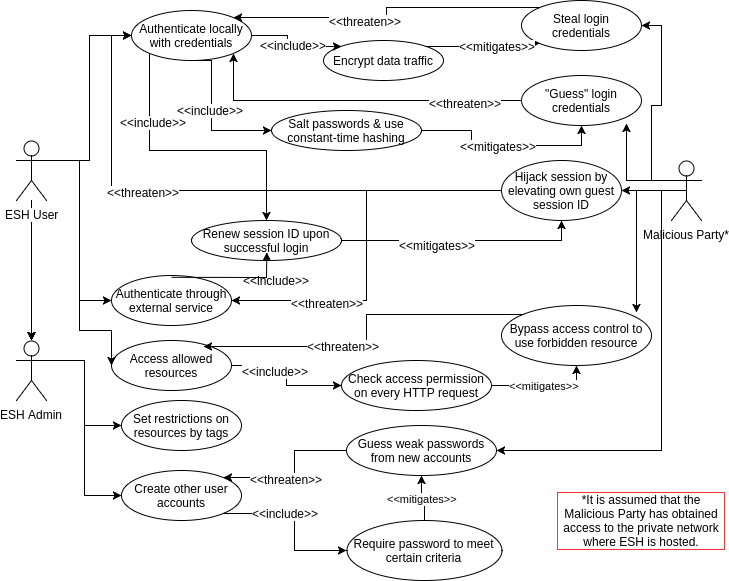
\includegraphics[width=\textwidth]{esh_misuse_cases}
\caption{Misuse Cases for Access Control in ESH.}
\label{fig:misuse_cases}
\end{center}
\end{figure}

\subsection{Proposed Token-Based Authentication Procedure}

On 15th February, 2018, a videocall meeting was held by the interested parties in the community with the purpose of clarifying the requirements gathered in the document mentioned in the subsection \ref{ssec:discussion}, and set priorities accordingly. Part of the discussion also meant to discuss how previously attempted solutions might be of use for the future implemention of authentication and access control. Among the most relevant agreed points was the use of JSON Web Tokens (JWT) to accomplish stateless authentication. The main reason for this decision was to reduce the effort needed to manage user sesions in the backend. It was also decided that the specifics of the access control mechanisms would be decided at a later point in time, since the most important priority was solving authentication. Therefore, further effort in this work focused on the implementation of a JWT-based authentication compatible with the Eclipse SmartHome architecture, and thus, compatible also with the openHAB software stack.

Typically, all kinds of token-based authentication follow these steps (REFERENCE):
\TODO{Structure as an algorithm}
\begin{enumerate}
\item The client sends its credentials (e.g. username, password, fingerprint) to the server.
\item The server attmpts to authenticate: if valid, it generates a token that includes expiration time.
\item The server stores a copy of the token and associates it with the user.
\item The server sends the token to the client.
\item In every future request, the client sends the token to the server.
\item For each request, the server extracts the token from the request, and looks up the user associated to it to perform authorization.
\item If the token is expired, the server generates a new token and sends it to the client. 
\end{enumerate}

The JSON Web Token (JWT) holds some peculiarities to other existing kinds of tokens. The primary difference is that this token includes a digital signature by the party that created it, e.g., the server. Thus, some adaptations would have to be applied to this procedure. Consider, for example, the limitations in the user interface in Eclipse SmartHome to provide web forms to put the credentials. For this reason, credentials are sent first through \emph{basic authentication}, since the web browser takes care of asking for the credentials. Therefore, the proposed authentication mechanism is as follows:

\TODO{Structure as an algorithm}
\begin{enumerate}
\item The client sends credentials through basic-authentication pop up form.
\item The server extracts credentials and, if these match a existing user, generate a JSON Web Token (JWT), appending to it the username and any additional fields, including expiration time and the server's digital signature of the JWT digest. Server sends the JWT to the client.
\item The client attaches the JWT on any future request.
\item For every request, the server extracts the JWT and verifies the digital signature. If valid, it takes the username and other claims, and performs authorization on the requested resource.
\item If the JWT is expired, the server requests credentials through basic-authentication, and if these are valid, it generates and serves a valid JWT.
\end{enumerate}

What may immediately stand out in this proposal, in contrast with the typical procedure is the embedding of the username as part of the JWT fields. Typically, a username is not considered to be \emph{confidential} and, although it normally isn't made public, it gives the adversary no significant advantage on stealing a user's data. In fact, if only resource access control is the goal, then the username does not need to be included. It would be sufficient to include the claims regarding the permissions on access to resources, since the validity of the token is relying on the signature. Moreover, for the sake of maintaining forward securtiy, a JWT is only renewed if the valid credentials are presented again. An adversary may, in some manner, retrieve an expired legitimate token. If this expired token would be presented to the server, then the server could present the adversary with a fresh token. Finally, the most important distinction is the use of digital signatures within the token. Indeed, if an adversary tried to impersonate a legitimate user through guessing usernames, it would not work, as the signature would not verify on the server's end. The security of the signature is as strong as the security of the signature, which may be RSA-2048, for instance.

The aforementioned procedure was designed with the assumption that, at all times, an HTTPS connection is present and thus, communication is protected through the TLS protocol. Otherwise, credentials and JWTs could be intercepted at any time by an adversary. 

\subsection{Architectural Implications of Authentication}

As a multi-layered automation software solution, it is not trivial to implement authentication, no matter the type, so that all parts of the system are covered by it. Recall that in subsection \ref{ssec:discussion} it was stated that resources to restrict do not only involve things, but also many different aspects of the system. Moreover, the Eclipse Smarthome is designed according to the OSGi architecture, and thus all modules are maintained as \emph{bundles}. These bundles contain, among other things, typical Java servlets and REST endpoints. If the methods present inside these Java classes have to go through some kind of \emph{check} before being executed, then access control may be implemented. This subsection includes details on the architecture and current development affairs, but this is introduced only as a base to delve into the proposed solution for authentication with JWT.

The idea, in general, is that any incoming HTTP request would have to be caught before running whatever Java method it attempted to access. For typical OSGi applications, the use of \emph{filters} is most commonly encouraged. A filter is a mechanism that may be applied before or after a Java method is accessed. Thus, it becomes a natural choice to employ filters for the purpose of access control.

It turns out, however, that regular filters do not work for the methods involving REST endpoints, such as a GET operation to return a list of all connected devices. These methods are actually based on the JAX-RS specification for a REST API in Java. In short, they require a different type of filters, which use a set of classes different from the regular OSGi filters. Aditionally, to make use of JAX-RS in OSGi applications, it is needed to use a third-party connector. Previous work on authentication for the Eclipse SmartHome made use of this connector and the special filters. There were problems with using these special filters, however: firstly, the permissions could only be set in the code, thus not appropriate for managing permissions at a more granular scale; secondly, due to classloading problems, it is a problem in some scenarios to make use of the JAX-RS third-party connector; and finally, this special filter is not compatible with traditional servlets (i.e., those that do not involve the JAX-RS REST API).

As part of the OSGi version 6 specification, filters may be registered to any resource through a special mechanism called the ``whiteboard pattern''. Current implementation of the Eclipse SmartHome runtime is bounded by the OSGi 4.2 specification, and it due to constraints in the rest of the software stack, it is not immediately possible to update to an implementation of the newer specification. Part of the work by the community was to create a \emph{bridge} between the OSGi 4.2 runtime and the newer whiteboard pattern functionality. For some time, this work focused on implementing JWT authentication for a ficticious, patched runtime. However, it was later decided that this bridge was not trivial, and halted development.

As development of the Eclipse Smarthome halted, a new direction involving traditional servlet security was considered for this work. As part of servlet registration to the OSGi runtime, an entity called \texttt{HttpContext} has to be provided. This entity provides the means to intercept HTTP requests before they reach the servlet, and thus it becomes the point where authentication and authorization may be implemented. Originally, this approach was discarded because the REST endpoints did not support the use of \texttt{HttpContext} alongside its registration. The key in this case is that both groups of servlets, the traditional and the REST servlet, run under different application contexts. What this means is that, even if a traditional servlet handles authentication properly, this information would not be propagated to the REST endpoints, and thus authorization mechanisms would not be enforced. In the months of March and April, however, part of the community started an effort to combine, or rather, to \emph{share} the provided \texttt{HttpContext} among servlets and REST endpoints.

Figure \ref{fig:esh_auth_arch} shows at a very high level the underlying architecture of the Eclipse SmartHome runtime. At the lowest level, the Jetty HTTP server and servlet engine is running. On top of it, there are several servlets running separately. Part of these servlets may be associated as being \emph{traditional}, while a particular servlet, the REST servlet, runs under different conditions. The REST servlet is used to serve resources, such as things, items, channels, etc. The Chart and Icon servlets, are of the traditional kind and thus, run under the same shared application context. Meanwhile, the REST servlet is shown to run under an isolated application context. Thus, the solution worked on by the community is to bridge both contexts and therefore have a commonly shared \texttt{HttpContext}. Yellow boxes represent the entities or resources that should have its access restricted according to a specified policy. Green boxes represent the possible solution to the problem, whereas the red boxes are the attempted solutions in previous years. Particularly, ``JAX-RS Custom ContainerContext'' was an attempted solution by the community, which had many problems when ported into the actual openHAB product. An alternative solution to it, the ``JAX-RS Custom Filter'' was originally planned to be implemented for this work, but the notion was discarded after understanding the limitations of this kind of filter, since it would not enforce authorization for the rest of the servlets (e.g. Icon servlet). 

\begin{figure} [ht] 
\begin{center}
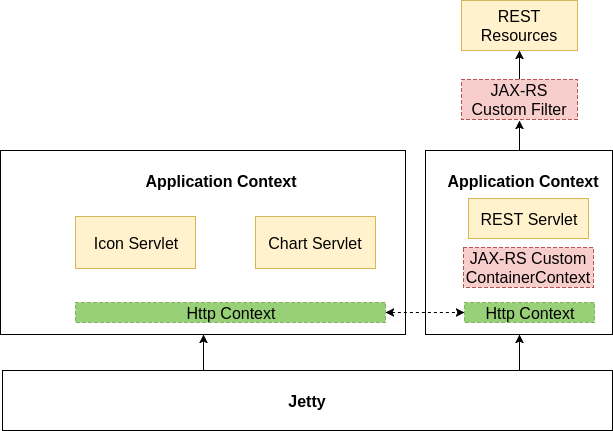
\includegraphics[width=0.8\textwidth]{esh_auth_arch}
\caption{Architecture breakdown into servlets.}
\label{fig:esh_auth_arch}
\end{center}
\end{figure}

Initial results by the community (REFERENCE) showed that it was indeed possible to make the \texttt{HttpContext} shared by the components that needed access control. Taking these results into account, work in the direction of a \emph{custom} \texttt{HttpContext} started. For this, the merged \texttt{HttpContext} will require the existence of an authenticator, i.e. a module that performs the authentication logic, and thereafter the module that performs authorization. Figure \ref{fig:esh_arch_authenticator} shows how the authenticator is merely a black box that may choose to perform a certain kind of authetnication according to the circumstance. The decision is based on the received HTTP request: depending on whether if has an authorization header, and if it does, which kind of authentication it intends to perform, or otherwise if there is a session identifier (cookie) present. Implementation details for the basic and JWT authenticators are introduced in subsection \ref{ssec:impl}. Form authentication is left as future work. 

\begin{figure} [ht] 
\begin{center}
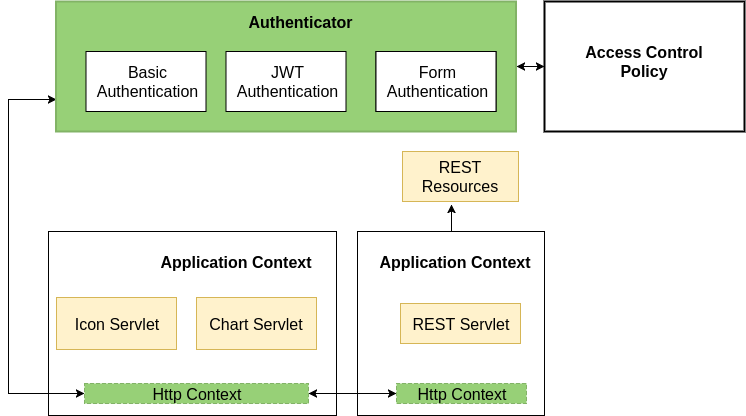
\includegraphics[width=0.8\textwidth]{esh_arch_authenticator}
\caption{Addition of authenticators into the architecture.}
\label{fig:esh_arch_authenticator}
\end{center}
\end{figure}

After the process of authentication, what follows is authorization. The authorization itself depends on the access control policies decided for the particular resources. This work focuses on authentication, and thus does not include the implementation of a particular access control policy. However, a proposal for access control is made in subsection \ref{ssec:autho}.

\subsection{Implementation of Authenticators}
\label{ssec:impl}

To model the sequence of events ocurring during the intended authentication procedure, a sequence diagram was written and is shown in figure \ref{fig:esh_auth_sequence}. This is showing the most compelling scenario: where the client interacts the first time with a servlet to get access to a resource. Clearly, as no credentials are provided at this time, the servlet requests basic authentication, and from there it generates a JSON Web Token (JWT). This token is used in any subsequent requests by the client. Note that the authorization policy is not included into this sequence of events. Thus, authorization becomes a binary aspect: if credentials are valid, then access is granted to the resource, regardless of its nature. Due to simplification, this diagram is only considering the use of valid credentials. In the actual implementation, invalid credentials result in a ``Forbidden Access'' response. 

\begin{figure} [ht] 
\begin{center}
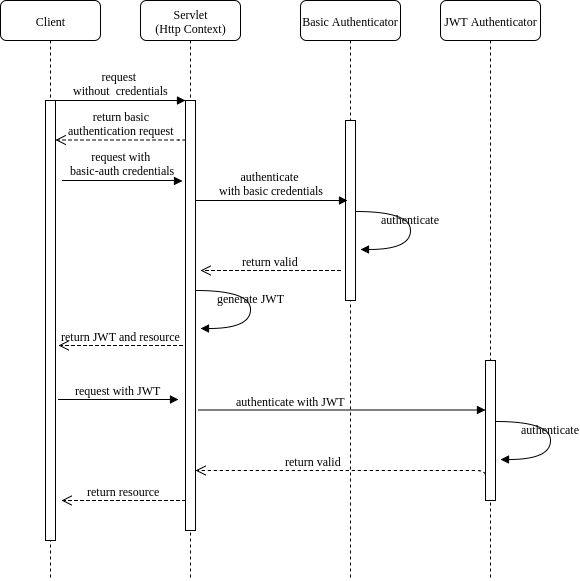
\includegraphics[width=0.8\textwidth]{esh_auth_sequence}
\caption{Authentication sequence diagram.}
\label{fig:esh_auth_sequence}
\end{center}
\end{figure}

The implementation of the authenticators was made into the \texttt{auth} bundle of the Eclipse SmartHome OSGi architecture. Due to the hierarchical nature of this project, many details will be omitted.  The core of the authenticator is located as part of the \texttt{CustomHttpContext} code located in this bundle.

As an interface class of the \texttt{Http Service} OSGi feature, \texttt{HttpContext} includes a method \texttt{handleSecurity} which, as the name implies, handles the security for the specified request to the servlet. As long as the servlet is registered with the custom \texttt{HttpContext}, every request into the servlet will go through the \texttt{handleSecurity} method.

\TODO{FIX HYPHEN ISSUES AND REF TO CODE SNIPPET INSTEAD OF FIG}
\begin{figure} [htb]
  \begin{lstlisting}
class CustomHttpContext implements HttpContext {   
 boolean handleSecurity(request,response) {
  if(request.getHeader("Authorization") == null \
       && request.getHeader("Cookie") == null) {
    response.addHeader("WWW-Authenticate", \
	"Basic realm=\"Test Realm\"");
    response.sendError(HttpServletResponse.SC_UNAUTHORIZED;
    return false;
  }	    
  if(jwtAuthenticated(request)) {
    return true;		
  } else if(basicAuthenticated(request)){
    username = getUsername(request);
    freshToken = generateJwt(username);
    response.addHeader("Set-Cookie", freshToken);
    return true;
  } else {
    response.sendError(HttpServletResponse.SC_UNAUTHORIZED);
    return false;
  }
 }
}
\end{lstlisting}
\caption{Core implementation of \texttt{CustomHttpContext}.}
\label{lst:core_impl}
\end{figure}

The simplified code snippet shows the core part of the \texttt{HttpContext} that intercepts requests and performs authentication from the provided HTTP header. As shown in the code snippet, after the JWT has been generated, it is given to the client as a \emph{cookie}. This way, no logic has to be implemented to manage the token in the client side (e.g. through local storage using HTML5). In subsequent requests, the cookie is presented to the server, and from it, the token is extracted and verified.

To handle the creation and verification of JWT, a third library library, Nimbus, was used (REFERENCE). This library even provides more complex features such as encryption of the JWT via a symmetric key encryption, but these are not currently considered for this work. As part of the basic structure of the JWT, a signature of the host is included at the end of the claims (e.g., username, permissions). For the proof of concept, an RSA-1024 key is generated as a singleton during runtime. Using the singleton pattern ensures that multiple private keys do not exist simultaneously, which could cause conflicts during signature verification. The freshly created RSA key is then used to both generate and sign the JWT, as shown in the simplified code snippet \ref{lst:rsa}.

\begin{figure} [htb]
\begin{lstlisting}
  protected String generateJwt(String username, String claim) {
    RSAPublicKey publicKey = (RSAPublicKey)getKeyPair().getPublic();
    RSAPrivateKey privKey = (RSAPrivateKey)getKeyPair().getPrivate();
    JWSObject jwsObject = new JWSObject(
    new JWSHeader.Builder(JWSAlgorithm.RS256).keyID("123").build(),
    new Payload(username));
    jwsObject.sign(new RSASSASigner(privKey));
    return jwsObject.serialize();	
  }    
\end{lstlisting}
\caption{Generation and signing of JWT.}
\label{lst:rsa}
\end{figure}

Code for the verification of the JWT is omitted as it follows a very similar logic to JWT generation and signing, but in reverse order. This implies de-serializing the JWT, loading the RSA public key into some object, verifying JWT using said object, and finally extracting username and claims. In the implementation, the username need not be extracted, as it is guaranteed that the claims are valid, given that the signature is valid.

As mentioned, the RSA key is generated at runtime once. Originally, this was meant to merely be a placeholder for a pre-existing RSA key that is present in the distribution of openHAB for SSH access. This pre-existing RSA key is stored in a file \texttt{keys.properties} under the \texttt{etc/} directory of the installation path of openHAB. However, it turned out that some problems emerged from this idea. First, the pre-existing RSA key was disabled, i.e. commented, as a security precaution. Secondly, the key is only generated as part of running the Karaf container inside the openHAB distribution. As Karaf is not included within the Eclipse SmartHome distribution, there is no pre-existing key. For the first problem, it would be enough to have the openHAB administrator generate a fresh key pair and store the public and private keys. However, this is not exactly user-friendly, and thus becomes a problem in terms of security usability.  A possible solution to the second problem is to leave key generation to the \texttt{auth} bundle and store it in some file in the local filesystem. When the bundle is activated it will first look for the file before attempting to generate a new RSA key. As the discussion within the community has not gotten to this point, the implementation has maintained the idea of storing the RSA key in memory during runtime. It should not cause problems and, in case that the bundle is restarted, then due to invalid JWTs, credentials will be requested again.

The rest of the implementation follows the authentication logic for the basic and token-based types. The code is currently maintained as a fork of the Eclipse SmartHome project (REFERENCE).
  
\subsection{Proposed Authorization Model}
\label{ssec:autho}
\TODO{Mention what will be "secured": servlets, REST endpoints, to view and to modify, etc}
As part of the access control mechanism, authorization is split up in several phases: defining a security policy, selecting an authorization model, implementing the model, and enforcing the policy (REFERENCE). As a smart home automation software, it is not trivial to define a security policy that covers all cases, due to the dynamic and varied-purpose devices present. The implementation of any authorization model emcompasses engineerning work tightly related to the OSGi architecture of the system, and thus, is left out of the scope of this work. However, by having knowledge of the resources that need to be restricted through access control, e.g. things, items, channels, system settings, an authorization model can be proposed independently of the authorization policy and implementation. Then, when a specific policy is decided by the Eclipse SmartHome community, the model will not change drastically, and thus, implementation can follow. 

For a smart home application, the focus of an authorization model should lean towards privacy-preservation and usability (REFERENCE). Considering that most end users of the openHAB are not tech-savvy, some options for an authorization model are instantly discarded. Some models are considered to be complex to manage and set up, such as the Attribute-Based Acess Control (ABAC), Usage Control (UCON), and the Access Control Matrix and List (ACM, ACL).

According to the requirements document written by the Eclipse Smart Home community, fine-grained access control is desired (REFERENCE). This is, an end user should be allowed to manage Things individually for each registered user, along with permissions regarding the sitemaps (User Interface templates), system settings, among others. An excellent fine-grained authorization model is the Attribute-Based Access Control. This model, however leaves a lot to be desired in terms of usability due to the management of every single permission as attributes for every user. This kind of management might end up in user pains, opting users to disable access control for the sake of comfort. 

Initially, it was considered to make direct use of the Role-Based Access Control (RBAC) authorization model. However, this kind of model works best when there are functional differences between the users of the system. In the case of openHAB, all users are typically members of the same household or temporal guests. In that sense, it does not make much sense to have a functional separation between users. However, it is reasonable to assume that some members of the household may not have the same rights as others. For example, a guest could be allowed to turn on/off the light switch, but may not be allowed to freely open the front door anytime. Likewise, permissions might not be equally split even among the permanent residents.

It was observed that the difference between users depend not on roles, but rather on the capabilities owned by each subject. The Capability-Based Access Control (CapBAC) overlaps with the idea of dynamically managing capabilities by granting some kind of token that describes these capabilities (REFERENCE). At first, it seems that this idea better fits with the needed authorization model for openHAB due to the flexibility to define permissions according to the capabilities of an entity. This notion is disolved when the implications of CapBAC are further analyzed, however. The authorization that CapBAC seeks to enforce is continous, that is, authorization is checked befure, during, and afterward access to a resource is requested. This particularity is meant to serve for the dynamic nature of the general IoT environment. However, for openHAB, a smart home application, the dynamic nature of smart devices is bounded by the the application itself: a single household.

An authorization model that makes use of the concept of roles as in the RBAC model and that focuses on capabilities, is described as follows. Consider a set of activities or tasks that may be performed on the Eclipse SmartHome, and consequently, the openHAB distribution. These tasks may vary from viewing or changing the status of a device connected to the system, to accessing certain parts of the sitemaps that serve as the user interface templates. These tasks may be grouped together as capability sets. For instance, the capability set ``speakers-playback'' may include actions such as modifying the speakers volume and even stopping or changing the track currently playing. Meanwhile, the capability set ``speakers-quiet'' may allow access to viewing the track currently playing and decreasing the speakers volume, for example. Consider a collection of different capability sets designed in advance for every \emph{type} of Thing, usually encompassed by a \emph{binding} in the Eclipse SmartHome. Finally, every user may be assigned a different collection of capability sets, thus making the permissions apparent and transparent. In that sense, a set of capabilities is akin to the concept of role in the RBAC model, and every user is assigned one or more roles, according to the actions permitted to them.

Table \ref{tbl:autho_cap} shows a sample assignment of capability sets to some users. Every user is expected to have at least one capability set, which may inherently encompass a number of permissions for the system. Table \ref{tbl:autho_op} offers an example that details the operations that access would be permitted for a particular capability set. For instance, a user with the \emph{things-all} capability set would have access to the REST resource that returns a JSON of all existing Things, as well as access to the method that allows registering a new Thing to the ecosystem. Thus, the proposed authorization model inspired by both the RBAC and CapBAC is a sound solution for the access management needs required of the Eclipse SmartHome and openHAB automation ecosystem. 

\begin{table}[h]
  \centering
  \begin{tabular}{|l|l|}
    \hline
    \multicolumn{1}{|c|}{\textbf{User}} & \multicolumn{1}{c|}{\textbf{Capability Sets}}            \\ \hline
    Marian                              & (speakers-quiet, lights-on, doors-close, sitemaps-paper) \\ \hline
    Erika                               & (speakers-playback, lights-all, doors-all, sitemaps-all) \\ \hline
  \end{tabular}
  \caption{Sample relation of user and capability sets}
  \label{tbl:autho_cap}
\end{table}

\begin{table}[h]
  \centering
  \begin{tabular}{ll}
    \hline
    \multicolumn{1}{|c|}{\textbf{Capability Set}} & \multicolumn{1}{c|}{\textbf{Involved Operations}}                                                                                                                                                                                      \\ \hline
    \multicolumn{1}{|l|}{speakers-playback}   & \multicolumn{1}{l|}{\begin{tabular}[c]{@{}l@{}}yamahareceiver.internal.state.\\NavigationControlState.getCurrentItemName()\\ ZoneControlState.volume\end{tabular}} \\ \hline
    \multicolumn{1}{|l|}{things-all}          & \multicolumn{1}{l|}{\begin{tabular}[c]{@{}l@{}}rest.core.internal.thing.ThingResource.getAll()\\ rest.core.internal.thing.ThingResource.create()\end{tabular}}                       \\ \hline
    &
  \end{tabular}
  \caption{Sample listings of operations involved for each capability set}
  \label{tbl:autho_op}
\end{table}

The proposed authorization model fulfills the purpose noted at the beginning of this subsection: satisfying security usability and somewhat-grained access control. Through the assignation of capability sets, an end user is capable of setting the permissions without causing significant pains. Additionally, through the definition of the operations involved in a capability set, the developer of a particular binding or component of Eclipse SmartHome or openHAB is able to implement the access control policy.

\newpage
\section{Evaluation}
\label{sec:eval}
\TODO{Short description of what this section is about}

\newpage
\section{Conclusion}
\label{sec:conclusion}
\TODO{what did you do?} 
\TODO{What are the results?}
\TODO{future work?}

\newpage
\section{Extra}
\subsection{How to use references} \label{sec:using_ref}

\paragraph{Cross-references to figures, tables and other document elements.}
LaTeX  internally numbers all kind of objects that have sequence numbers:
\begin{itemize}
\item chapters, sections, subsections;
\item figures, tables, algorithms;
\item equations, equation arrays.
\end{itemize}
To reference them automatically, you have to generate a label using \texttt{$\backslash$label\{some-name\}} just after the object that has the number inside. Usually, labels of different objects are split into different namespaces by adding dedicated prefix, such as \texttt{sec:}, \texttt{fig:}. To use the corresponding reference, you must use command \texttt{$\backslash$ref} or \texttt{$\backslash$eqref}. For instance, we can reference this subsection by calling Section~\ref{sec:using_ref}. Note that there should be a nonbreakable space \texttt{\~} between the name of the object and the reference so that they would not appear on different lines (does not work in Estonian).          


\paragraph{Citations.}
Usually, you also want to reference articles, webpages, tools or programs or books. For that you should use citations and references. The system is similar to the cross-referencing system in LaTeX. For each reference you must assign a unique label. Again, there are many naming schemes for labels. However, as you have a short document anything works. To reference to a particular source you must use \texttt{$\backslash$cite\{label\}} or \texttt{$\backslash$cite[page]\{label\}}. 

References themselves can be part of a LaTeX source file. For that you need to define a bibliography section. However, this approach is really uncommon. It is much more easier to use BibTeX to synthesise the right reference form for you. For that you must use two commands in the LaTeX source
\begin{itemize}
\item $\backslash$bibliographystyle\{alpha\} or $\backslash$bibliographystyle\{plain\}
\item $\backslash$bibliography\{file-name\}
\end{itemize}
The first command determines whether the references are numbered by letter-number combinations or by cryptic numbers. It is more common to use \texttt{alpha} style. The second command determines the file containing the bibliographic entries. The file should end with \texttt{bib} extension. Each reference there is in specific form. The simplest way to avoid all technicalities is to use graphical frontend  Jabref (\url{http://jabref.sourceforge.net/}) to manage references. Another alternative is to use DBLP database of references and copy BibTeX entries directly form there.   
    
   
The following paragraph shows how references can be used. Game-based proving is a way to analyse security of a cryptographic protocol~\cite{GameB_1, GameB_2}. There are automatic provers, such as {CertiCrypt\-}~\cite{dummy} and ProVerif~\cite{proVerif}.


\newpage
\section{How to add figures and pictures to your thesis}


Here are a few examples of how to add figures or pictures to your thesis (see Figures~\ref{fig:fnCompModel}, \ref{fig:game-based_proofs}, \ref{fig:proveit_screenshot}).

Rule: All the figures, tables and extras in the thesis have to be referred to somewhere in the text.


\begin{figure} [ht] %try to place the figure here (next option top of the page) 
\begin{center}
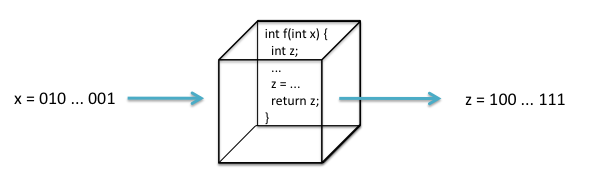
\includegraphics[width=0.8\textwidth]{computational_model_function}
\caption{The title of the Figure.}
\label{fig:fnCompModel}
\end{center}
\end{figure}



\begin{figure} [!ht] %if [h] doesn't work, we can force with !
\begin{center}
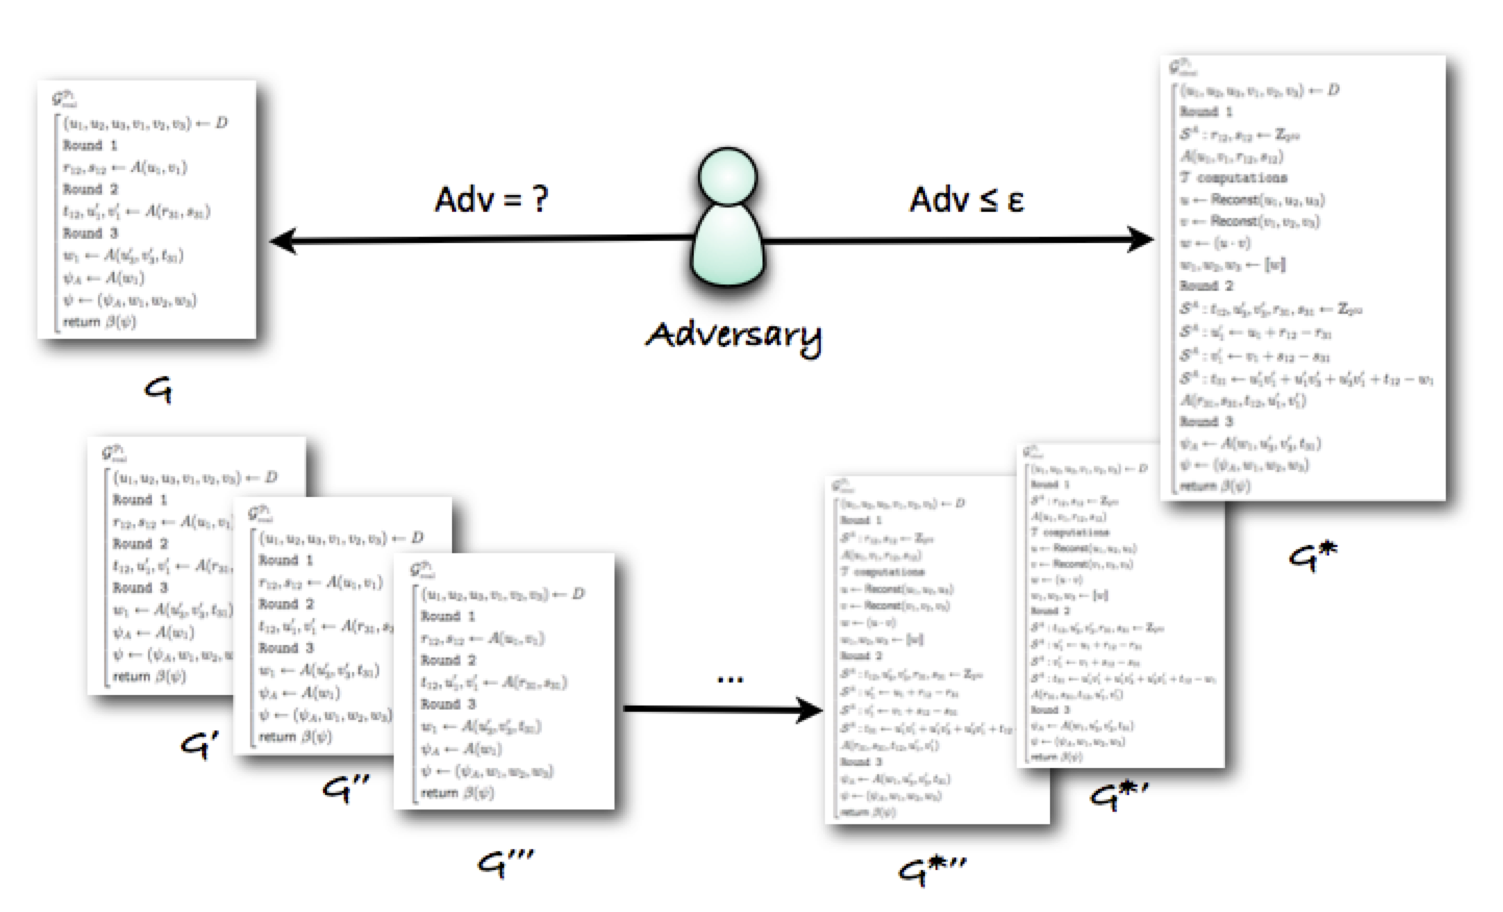
\includegraphics[width=\textwidth]{game-based_proofs}
\caption{Refer if the figure is not yours~\cite{kamm12}.}
\label{fig:game-based_proofs}
\end{center}
\end{figure}


\begin{figure} [p]
\begin{center}
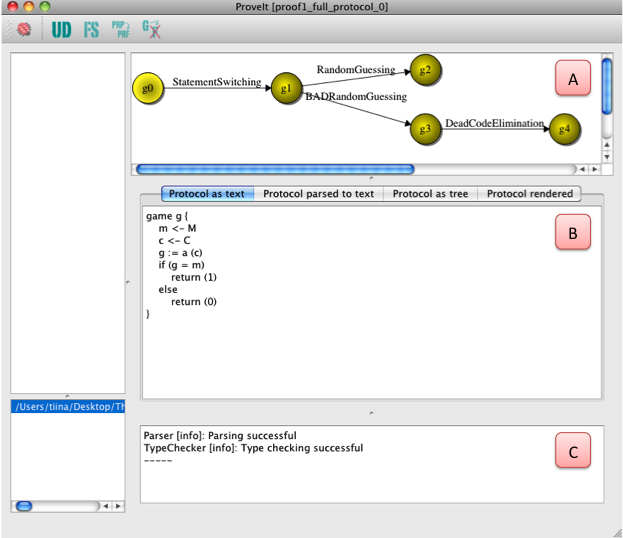
\includegraphics[width=\textwidth]{proveit_screenshot}
\caption{Screenshot of \proveit.}
\label{fig:proveit_screenshot}
\end{center}
\end{figure}

Tip: If you add a screenshot then labeling the parts might help make the text more understandable (panel C vs bottom left part), e.g.


\begin{figure} [htbp]
\begin{tabular}{c c}
%
\begin{minipage}{0.45\textwidth}
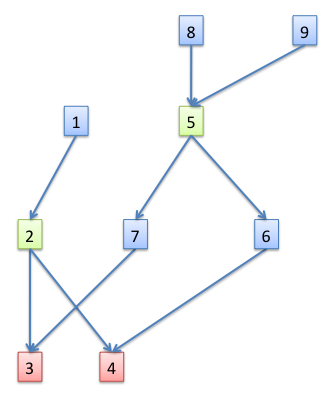
\includegraphics[width=\textwidth]{LCA_2_solutions}
\end{minipage}
%
&
\begin{minipage}{0.55\textwidth}
\centering
\begin{tabular}{ l | l |}
	Node & Decendants \\ \hline
  1 & 2, 3, 4 \\ \hline
  2 & 3, 4 \\ \hline
  3 & \\ \hline
  4 & \\ \hline
  5 & 3, 4, 6, 7 \\ \hline
  6 & 4 \\ \hline
  7 & 3 \\  \hline
  8 & 3, 4, 5, 6, 7\\ \hline
  9 & 3, 4, 5, 6, 7\\ \hline
\end{tabular}
\end{minipage}
\end{tabular}
%
\caption{Example how to put two figures parallel to each other.}
\label{fig:LCA_2_solutions}
\end{figure}


Example: A screenshot of \proveit can be seen on Figure~\ref{fig:proveit_screenshot}. The user first enters the pseudocode of the initial game in panel B. \proveit also keeps track of all the previous games showing the progress on a graph seen in panel A.

There are two figures side by side on Figure~\ref{fig:LCA_2_solutions}.



\clearpage %if newpage doesn't work
\section{Other Ways to Represent Data}

\subsection{Tables}

\begin{table}[h]
\centering
\caption{Statements in the \proveit language.}
\begin{tabular}{| l | l |}
	\hline
	\bf{Statement} & \bf{Typeset Example} \\
	\hline
	assignment & $a := 5 + b$ \\
	\hline
	uniform choice & $m <- M$ \\
	\hline
	function signature & $f : K \times M -> L$\\
	\hline
\end{tabular}
\label{tab:statements}
\end{table}


\subsection{Lists}

Numbered list example:
\begin{enumerate}
	\item item one; 
	\item item two;
	\item item three.
\end{enumerate} 

\subsection{Math mode}
Example:
\begin{equation}
a + b = c + d
\end{equation}
Aligning:
\begin{align*}
	a &= 5 \\
	b + c &= a \\
	a -2*3 &= 5/4
\end{align*}
Hint: Variables or equations in text are separated with \$ sign, e.g. $a$, $x - y$.

\paragraph{Inference Rules}
\[ 
	\inference[addition]{x : T & y : T}{x + y : T} 
\]
Bigger example:
\[
\inference[assign]{c := a + b & 
	\inference[addG]{a : \typeRat & 
		\inference[var]{b : \typeInt & \typeInt \subseteq \typeRat}{b : \typeRat}
		}{a + b : \typeRat}
	}{c : \typeRat}
\]


\subsection{algorithm2e}

\begin{algorithm} [!h]
	\caption{typeChecking} \label{alg:typeChecking}
	\KwIn{Abstract syntax tree}
	\KwResult{Type checking result; In addition, type table \typeF{type\_G} for global variables, \typeF{game} for the main game and \typeF{fun} for each $fun \in F$}
	\SetKwData{s}{s}
	\BlankLine
	
	\While{something changed in last cycle}{
		\lForEach{global statement \s} {
			\parseStatement{\s, \typeF{type\_G}}\;
		}
		\ForEach{function $fun$} {
		\lForEach{statement \s in $fun$} {
			\parseStatement{\s, \typeF{fun}}\;
		}
		}
		\lForEach{statement \s in game} {
			\parseStatement{\s, \typeF{game}}\;
		}
	}
	%\eIf{error messages were found}{\Return \False\;}{\Return \True\;}
\end{algorithm}

\subsection{Pseudocode}

\begin{figure} [htb]
\begin{lstlisting}
expression
  : NUMBER
  | VARIABLE
  | '+' expression
  | expression '+' expression
  | expression '*' expression
  | function_name '(' parameters ')'
  | '(' expression ')'
\end{lstlisting}
\caption{Grammar of arithmetic expressions.}
\label{fig:parser_exp}
\end{figure}

\subsection{Frame Around Information}

Tip: We can use minipage to create a frame around some important information.
\begin{figure} [h]
\frame{
\begin{minipage}{\textwidth}
\begin{enumerate}
	\item integer division ($\opDiv$) -- only usable between \typeInt types
	\item remainder ($\%$) -- only usable between \typeInt types
\end{enumerate}
\end{minipage}
}
\caption{Arithmetic operations in \proveit revisited.}
\label{fig:aritmOp_revisit}
\end{figure}

\newpage

% BibTeX bibliography
\bibliographystyle{alpha} %plain=[1], alpha=[BGZ09]
\bibliography{master-thesis}

\addcontentsline{toc}{section}{\refname}


% Use Biblatex if you have problems with Estonian keywords
%\printbibliography %biblatex


% Use alternative local LaTeX bibliography
\begin{comment}
\begin{thebibliography}{9}
\bibitem{proVerif} 
  Bruno Blanchet. 
  Proverif: Cryptographic protocol verifier in the formal model.
  \url{http://www.proverif.ens.fr/}.
  (checked 15.05.2012)
\bibitem{GameB_1} GameB1
\bibitem{GameB_2} GameB2
\bibitem{dummy} dummy
\bibitem{kamm12} kamm12
\end{thebibliography}
\end{comment}


\newpage
%\appendix
%\section*{\appendixname}
\iflanguage{english}%
  {\section*{Appendix}
  \addcontentsline{toc}{section}{Appendix}
  }%
  {\section*{Lisad}
  \addcontentsline{toc}{section}{Lisad}}


\section*{I. Glossary}
\addcontentsline{toc}{subsection}{I. Glossary}
Bearer token. The digest of the user credentials to be used in an authentication process.
Manifest. Configuration file for OSGi bundles that define the bundle's unique identification, packages imported from other bundles, and packages to make available to other bundles.
\newpage

%=== Licence in English
\newcommand\EngLicence{{%
\selectlanguage{english}
\section*{II. Licence}

\addcontentsline{toc}{subsection}{II. Licence}

\subsection*{Non-exclusive licence to reproduce thesis and make thesis public}

I, \textbf{Jes\'{u}s Antonio Soto Vel\'{a}zquez},

\begin{enumerate}
\item
herewith grant the University of Tartu a free permit (non-exclusive licence) to:
\begin{enumerate}
\item[1.1]
reproduce, for the purpose of preservation and making available to the public, including for addition to the DSpace digital archives until expiry of the term of validity of the copyright, and
\item[1.2]
make available to the public via the web environment of the University of Tartu, including via the DSpace digital archives until expiry of the term of validity of the copyright,
\end{enumerate}

of my thesis
\textbf{Security of the openHAB Smart Home}

supervised by Satish Narayana Srirama and Danilo Gligoroski

\item
I am aware of the fact that the author retains these rights.
\item
I certify that granting the non-exclusive licence does not infringe the intellectual property rights or rights arising from the Personal Data Protection Act. 
\end{enumerate}

\noindent
Tartu, 21.05.2018
}}%\newcommand\EngLicence


%=== Licence in Estonian
\newcommand\EstLicence{{%
\selectlanguage{estonian}
\section*{II. Litsents}

\addcontentsline{toc}{subsection}{II. Litsents}

\subsection*{Lihtlitsents lõputöö reprodutseerimiseks ja lõputöö üldsusele kättesaadavaks tegemiseks}

Mina, \textbf{Jes\'{u}s Antonio Soto Vel\'{a}zquez},

\begin{enumerate}
\item
annan Tartu Ülikoolile tasuta loa (lihtlitsentsi) enda loodud teose

\textbf{Tüübituletus neljandat järku loogikavalemitele}

mille juhendajad on Satish Narayana Srirama ja Danilo Gligoroski

\begin{enumerate}
\item[1.1]
reprodutseerimiseks säilitamise ja üldsusele kättesaadavaks tegemise eesmärgil, sealhulgas digitaalarhiivi DSpace-is lisamise eesmärgil kuni autoriõiguse kehtivuse tähtaja lõppemiseni;
\item[1.2]
üldsusele kättesaadavaks tegemiseks Tartu Ülikooli veebikeskkonna kaudu, sealhulgas digitaalarhiivi DSpace´i kaudu kuni autoriõiguse kehtivuse tähtaja lõppemiseni.
\end{enumerate}


\item
olen teadlik, et punktis 1 nimetatud õigused jäävad alles ka autorile.
\item
kinnitan, et lihtlitsentsi andmisega ei rikuta teiste isikute intellektuaalomandi ega isikuandmete kaitse seadusest tulenevaid õigusi. 
\end{enumerate}

\noindent
Tartus, 21.05.2018
}}%\newcommand\EstLicence


%===Choose the licence in active language
\iflanguage{english}{\EngLicence}{\EstLicence}


\end{document}

